
\section{Introduction}

Derivative free optimization (DFO) refers to mathematical programs involving functions for which derivative information is not explicitly available.
Such problems arise, for example, when the functions are evaluated by simulations or by laboratory experiments.
In such applications, function evaluations are expensive, so it is sensible to invest significant computational resources to minimize the number of function evaluations.

This work is ultimately aimed at developing algorithms to solve constrained optimization problems of the form 

\[ \begin{array}{ccl} \min_{x \in \domain} & f(x) \\
\mbox{subject to} & c_i(x) \le 0 & i \in \mathcal{I} \\
& c_i(x) = 0 & i \in \mathcal{E},
\end{array}
\]
where $\domain$ is a subset of $\real^n$, and $f$ and $c_i, i \in \mathcal{I} \cup \mathcal{E}$ are real-valued functions on $X$ with at least one of these functions being a {\em black-box} function, meaning that derivatives cannot be evaluated directly.

%%%%%%%%%%%%%%%%%%%%%%%%%%%%%%%%%%%%%%%%%%%%%%%%%%%%%%%%%%%%%%%%%%%%%%%%%%%%%%%%%%%%%%%%%%%%%%%%%%%%%%%%%%%%%%%%%%%%%%%%%%%%%%%%%%%%
% We consider two variations of this problem.
% In the first variation, we assume that the constraints are fully quantifiable.
%%%%%%%%%%%%%%%%%%%%%%%%%%%%%%%%%%%%%%%%%%%%%%%%%%%%%%%%%%%%%%%%%%%%%%%%%%%%%%%%%%%%%%%%%%%%%%%%%%%%%%%%%%%%%%%%%%%%%%%%%%%%%%%%%%%%

We are specifically interested in applications were some of the black box functions cannot be evaluated outside the feasible region.
As in \cite{DUMMY:typesofconstraints}, quantifiable means that the functions can be evaluated at any point in $X$ and that the values returned for the constraint functions provide meaningful information about how close the point is to a constraint boundary.
We assume that the black-box functions return meaningful numerical values \emph{only} when evaluated at feasible points.
In this case, the constraints are called {\em partially quantifiable}.   
As such, we impose the requirement that all sample  points must be feasible.

We are interested in developing {\em model-based} trust-region algorithms for solving these problems.
Model-based methods work by constructing model functions to approximate the black box functions at each iteration.
The model functions are determined by fitting previously evaluated function values on a set of sample points.
In trust-region methods, the model-functions are used to define a trust-region subproblem, whose solution determines the next iterate.
For example, the trust-region subproblem might have the form

\[ \begin{array}{ccl} \min_{\norm{s} \le \Delta_k}
 & \modelk (\iteratek+s) \\
\mbox{subject to} & \modelconstrainti(\iteratek + s) \le 0 & i \in \mathcal{I} \\
& \modelconstrainti(\iteratek + s) = 0 & i \in \mathcal{E},
\end{array}
\]
where $\iteratek$ is the current iterate, $\modelk$ is the model function approximating $f$,  and $\modelconstrainti$ are the model functions approximating the constraint $c_i \forall i \in \mathcal{I} \union \mathcal{E}$, and $\Delta_k$ is the radius of the trust-region.
The key differences between this problem and the original is that all functions are replaced with their model functions, and a trust region constraint has been added.
Conceptually, the model functions are ``trusted'' only within a distance $\Delta_k$ of the current iterate $\iteratek$; so the trust-region subproblem restricts the length of step $s$ to be no larger than $\Delta_k$.
To ensure that the model functions are good approximations of the true functions over the trust region, the sample points are typically chosen to lie within, or at least near, the trust-region.


An important consideration in fitting the model functions is the ``geometry'' of the sample set.
This will be discussed in more detail in Section \cref{geometry}, but the key point is that the relative positions of the sample points within the trust region have a significant effect on the accuracy of the model functions over the trust region.
When the geometry of the sample set is poor, it is sometimes necessary to evaluate the functions at new points within the trust region to improve the geometry of the sample set.

The requirement that all sample points are feasible poses some interesting challenges for the geometry of the sample set.
As a first step toward developing an algorithm to solve such problems, \emph{we consider a simplified problem where all of the constraints are linear}.

%%%%%%%%%%%%%%%%%%%%%%%%%%%%%%%%%%%%%%%%%%%%%%%%%%%%%%%%%%%%%%%%%%%%%%%%%%%%%%%%%%%%%%%%%%%%%%%%%%%%%%%%%%%%%%%%%%%%%%%%%%%%%%%%%%%%
% In the case of fully quantifiable constraints, there is no difficulty in using sample points outside of the feasible region.  
% In Chapter \cref{chap:Filter}, we describe a Trust-Region SQP Filter method for solving this class of problems.
%%%%%%%%%%%%%%%%%%%%%%%%%%%%%%%%%%%%%%%%%%%%%%%%%%%%%%%%%%%%%%%%%%%%%%%%%%%%%%%%%%%%%%%%%%%%%%%%%%%%%%%%%%%%%%%%%%%%%%%%%%%%%%%%%%%%
  
% 
% \subsection{Always Feasible Motivation}
% 
% Algorithms that maintain feasibility in both the iterates and sample points provide some useful qualities.
% Firstly, they are able to solve problems with \emph{partially-quantifiable} constraints.
% One scenario in which partially-quantifiable constraints may arise is within the problem of minimizing an expensive simulation.
% 
% %\begin{center}
% %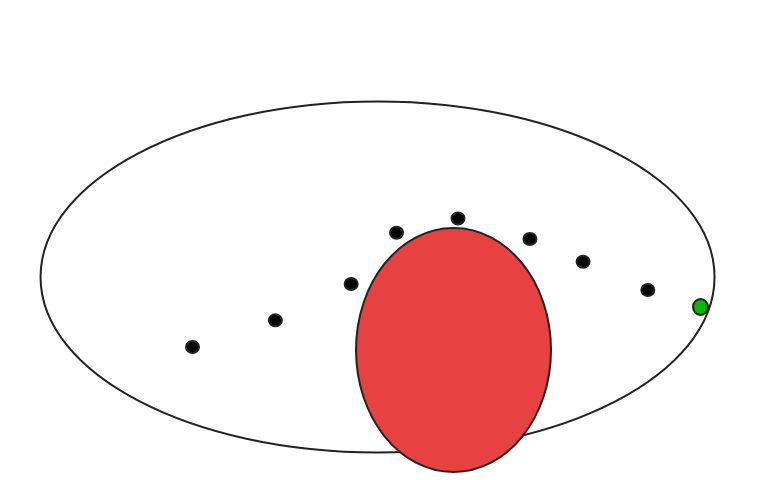
\includegraphics[width=200px]{images/infeasible_constraint.png}
% %\end{center}
% 
% If the runtime of the simulation depends on its inputs, and the simulation is not allowed to finish when a runtime threshold is met, the runtime will force some inputs to be infeasible.
% However, when the simulation does complete, its runtime is quantifiable, and can be used to construct a model of the infeasible region.
% An algorithm that wishes to minimize this simulation is forced to account for this constraint.
% 
% 
% An always feasible algorithm is also an \emph{any-time} algorithm.
% Anytime algorithms are a class of algorithms that can conveniently be run as long as desired and return the best solution found so far if interrupted.
% These algorithm are of practical importance when problems have uncertain time complexity.
% 

\subsection{Notation}

Any variables that depend on the iteration will be super-scripted by $k$.
For example, the $k$-th iterate is given by $\iteratek$, and the model of the objective is given by $\modelk$.
The $i$ row of the matrix $A$ is denoted $A_i$, while the $i$-th column is denoted $A_{\bullet i}$.
Subscripts on vectors are used as an index into the vector, while vectors in a sequence of vectors use superscripts.
Matrices are denoted with capital letters, and we use $e_i$ to denote the unit vector.                     %, while sets are denoted with capital italic letters.

$B_k(c; \Delta)$ is the ball of radius $\Delta$ centered at point $c$ in the $k$ norm.
Finally, $\delta_{i,j}$ is the kronecker delta function, $\delta_{i,i} = 1$, $\delta_{i,j} = 0$ if $i\ne j$.


\subsection{Model-based Trust Region Methods}

We will modify the following derivative free trust region algorithm.
%A set of poised points are chosen for some radius $\Delta_k>0$ about the current iterate.
The objective value and derivatives are approximated in a trust region around the current iterate to construct their model functions.
Next, this model function is minimized over the trust region and the minimum argument becomes the trial point.
The objective is evaluated at the trial point and a measure of reduction $\rho$ is computed.
If $\rho$ implies that sufficient reduction has been made and that the model approximates the function well, the trial point is accepted as the new iterate.
Otherwise, the trust region is reduced to increase model accuracy.
The algorithm terminates when both and a criticality measure $\chik$ and the trust region radius $\Delta_k$ reach sufficiently small thresholds of $\tau_{\chi}$ and $\tau_{\Delta}$.


For unconstrained optimization, the algorithmic framework is described in \cref{unconstrained_dfo}.
% 	\begin {itemize}
%         \item The objective is evaluated at a set of sample point $Y$ to approximate $f$ \cref{interpolation}
%         \item Geometric properties ensure bounds on $f(x) - \modelk(x)$, $\nabla f(x) - \gradmodelk(x)$, and $\nabla^2 f(x) - \nabla^2\modelk(x)\;\forall x$ in the trust region \cref{geometry}
% 		%\[
% 		%\modelk(x) = f(\iteratek) + \nabla f(\iteratek)^T (x-\iteratek) + \frac 1 2 (x-\iteratek)^T\nabla^2f(\iteratek)(x-\iteratek)
% 		%\]
% 		\item If $\rho$ is large, $\iteratekpone=\iteratek+\trialk$ (accept) and either increase the radius or decrease if $\nabla \modelk(\iteratek)$ is small
% \end{itemize}

\begin{algorithm}[H]
    \caption{Unconstrained Derivative Free Algorithm}
    \label{unconstrained_dfo}
    \begin{itemize}
        \item[\textbf{Step 0}] \textbf{(Initialization)} \\
            Initialize tolerance constants $\tau_{\chi} > 0$, $\tau_{\Delta} > 0$, starting point $x^{(0)}$, initial radius $\Delta_0 > 0$, iteration counter $k=0$, and constants $\omegadec \in (0, 1)$, $ \gammasm \in (0, 1)$, $\gammabi \in (\gammasm, 1)$.
            
        \item[\textbf{Step 1}] \textbf{(Construct the model function)} \\
            Call the model improvement ``\cref{model_improving_algorithm}" to provide a set of sample points $Y^{(k)}$.
            Evaluate the objective on these points and use interpolation \cref{interpolation_formula} to construct the model function $\modelk(x)$.
        
        \item[\textbf{Step 2}] \textbf{(Check stopping criteria)} \\
            Compute the criticality measure $\chik$ such as $\chik = \|\nabla\modelk(\iteratek)\|$. \begin{itemize}
                \item[] If $ \chik < \tau_{\chi} $ and $\Delta_k<\tau_{\Delta}$ then return solution $\iteratek$.
                \item[] If $ \chik < \tau_{\chi} $ but $\Delta_k\ge\tau_{\Delta}$ then  
                set $\Delta_{k+1} \gets \omegadec\Delta_{k}$, 
                $x^{(k+1)} \gets \iteratek$,
                $k \gets k+1$ and go to Step 1.
            \end{itemize}
        
        \item[\textbf{Step 3}] \textbf{(Solve the trust region subproblem)} \\
            Compute $\trialk = \argmin_{s\in B_2(0; \Delta_k)} \modelk (\iteratek + s)$ where $B_2(0; \Delta_k)$ is the ball of radius $\Delta_k$ defined in \cref{tab:TableOfNotation}.
            
        \item[\textbf{Step 4}] \textbf{(Test for improvement)} \\
            Compute $\rho$ with \cref{rho} \begin{itemize}
                \item[] If $\rho < \gammasm$ then $\iteratekpone \gets \iteratek$ (reject) and $\Delta_{k+1} \gets \omegadec\Delta_{k}$
                \item[] If $\rho \ge \gammasm$ and $\rho < \gammabi$ then $\iteratekpone\gets\iteratek+\trialk$ (accept) $\Delta_{k+1} \gets \omegadec\Delta_{k}$
                \item[] If $\rho \ge \gammabi$ and $\|\trialk\| = \Delta_{k}$ then $\iteratekpone=\iteratek+\trialk$ (accept) $\Delta_{k+1} \gets \omegainc\Delta_{k}$
                % and either increase the radius or decrease if $\nabla \modelk(\iteratek)$ is small
            \end{itemize}
            $k \gets k+1$ and go to Step 1.
    \end{itemize}
\end{algorithm}

This derivative-free optimization algorithm differs from the classical trust region algorithm in two important respects:
\begin{enumerate}
    \item Models are constructed without derivative information.
    \item The trust region radius $\Delta_k$ must go to zero as $k\to\infty$.
\end{enumerate}

These are required to ensure that the gradient of the model function is equal to the gradient of $f$ in the limit.
Our goal is to generalize this framework to handle constraints, where we must ensure no constraint violation occurs while also ensuring the accuracy of the models of the constraints.
% Two challenges while adopting this framework to derivative free optimization are
% 
% Because explicit derivatives are not available, Taylor approximations cannot be used.
% The alternative to Taylor approximations that we employ is interpolation.
% Also, classical trust region methods do not require $\Delta_k \to 0$, but the bounds on model accuracy in derivative free optimization depend on the trust region radius.
% This means that in order to ensure $\nabla f < c\tau$ using the approximation  $\nabla \modelk < \tau$, the trust region must be sufficiently small.
%   
  

\section{Derivative Free Background}
% 
% \subsection{Strategy}
% A reasonable approach to DFO is to modify classical algorithms that rely on derivatives by using the derivatives of the model functions whenever a derivative is needed in the algorithm.
% However, the lack of explicit derivatives pose several challenges, which necessitate changes in the classical algorithms.
% First, care must be taken to ensure that the model functions are sufficiently accurate approximations to the true functions.
% This means that geometry of the sample points must be considered.
% It also means that the trust-region radius must get arbitrarily small.
% 
% The transition to the derivative-free setting also provides some interesting research opportunities.
% In particular, because function evaluations are so costly, there is potential for significant gains by considering more complex optimization paradigms.
% For example, Sequential Quadratic Programming (SQP) methods use subproblems involving quadratic approximations of the objective function $f$ and linear approximations of the constraint functions.
% In the derivative-free setting, it may be worthwhile to explore other variations of the classical algorithms.
% For example, it might be worthwhile to construct quadratic models of the constraint functions, which might result in fewer iterations overall.
% 
% It might also be worthwhile to consider using different sample sets for fitting different functions.  
% For example, the SQP trust-region filter method involves constructing a quadratic model of the objective function and linear models of the constraint functions.  But this raises an interesting question, since a good sample set for constructing a quadratic model may not be ideal for fitting the linear functions modeling the constraints.  

\subsection{Recent Work}
\paragraph{Applications}
Recently, there has been a growth in applications of derivative free optimization.
Such applications include photo-injector optimization \cite{1742-6596-874-1-012062}, circuitry arrangements \cite{PLOSKAS201816}, machine learning \cite{KS2018}, volume optimization \cite{Cheng2017}, and reliability based optimization \cite{Gao2017}.

\paragraph{Constrained derivative free algorithms}
To address the rise in these applications, new algorithms are being developed such as \cite{doi:10.1080/10556788.2015.1026968} which is an algorithm similar to the one presented here, but the sample points are not always feasible.
\cite{Tröltzsch2016} presents another similar algorithm for equality based constraints.
\cite{infeasiblestarting} presents an algorithm which accepts an infeasible starting point.
\cite{Gao2018} also presents an algorithm for linearly constrained derivative free optimization that uses a backtracking technique to minimize the number of evaluations required.

\paragraph{Subproblems}
Some work has been done within trust region algorithms to improve the update policy \cite{Kamandi2017}.
Also, \cite{Verdério2017} and \cite{doi:10.1080/10556780802409296} discuss geometric conditions of the sample points required for global convergence.
Finally, \cite{AMAIOUA201813} uses a mesh adaptive search to solve quadratic subproblems.


\paragraph{Complexity Analysis}

A derivation is found in \cite{doi:10.1137/151005683} which shows that to driver the norm of the gradient less than $\epsilon$, the number of function evaluations can be bounded by $O(\epsilon^{-2})$ 
%and $O(n^2\epsilon^{-2})$ 
function evaluations for derivative free model based approaches. Also, cubic over estimation with finite differences can acheive $O(\epsilon^{-1.5})$. \cite{doi:10.1093/imanum/drx043} is another recent paper presenting complexity analysis using probabilistic methods.


\paragraph{Reviews}
Within \cite{DUMMY:intro_book} derivative-free methods are developed in detail.
This is the first text book devoted to derivative free optimization.
It contains a good explanation of ensuring geometry of the current set with poisedness for unconstrained problems and also covers other derivative-free methods including direct-search and line search.

A good review of derivative free algorithms and software libraries can be found in \cite{DUMMY:review}.
This compares several software libraries, and reviews the development of derivative free optimization since it started.
Another recent review can be found in \cite{DUMMY:review2}.

% TODOOOOOOOOOOOOOOOOOOOOOOOOOOOOOOOOOOOOOOOOOOOOOOOOOOOOOOOOOOOOOOOOOOOOOOOOOOOOOOOOOOOOOOOOOOOOOOOOOOOOOOOOOOOO
% READ THIS


\subsection{Sample Set Geometry}

\subsubsection{Sampling Issues}

Derivative free trust region methods construct model functions from a family of functions spanned by a set of $p \in \mathbb N$ basis functions 
$\{\phi_0, \phi_2, \ldots, \phi_p\}$.
Each member of this family has the from $\modelk(x) = \sum_{i=0}^p\alpha_i\phi_i(x)$ for some scalar coefficients $\alpha_i, i \in \{0, \ldots, p\}$.
In our method, we use interpolation to choose the coefficients so that $\modelk$ agrees with $f$ on a set of sample points $Y = \{y^0, y^1, \ldots, y^p\}$.
When this is done, care must be taken to avoid issues with their \emph{geometry}.

\paragraph{Interpolation}
\label{interpolation}
Suppose that we use $p+1$ sample points $Y = \{y^0, y^1, \ldots, y^p\}$ to construct the approximation of $f$.
We desire a method for choosing these sample points that provides error bounds on not only the function values, but also on orders of derivatives in some region around the current iterate.
The model is constructed to agree with the original functions on at least the sample points: we evaluate the objective here, so that we know the true function values at these points.
For the objective, this becomes
\begin{align}
\label{interpolation_condition}
\modelk(y^i) = f(y^i) \quad \forall \quad 0 \le i \le p.
\end{align}
This is known as the \emph{interpolation condition}.

It is convenient to write the model as a linear combination of basis polynomials $\{\phi_0, \phi_2, \ldots, \phi_p\}$.
To satisfy the interpolation condition \cref{interpolation_condition}, we then chose this linear combination by selecting coefficients $\alpha_0, \ldots, \alpha_p$ to satisfy
\begin{align}
\label{interpolation_formula}
    \modelk(y^i) = \sum^p_{j=0}\alpha_j\phi_j(y^i) = f(y^i) \quad \forall \quad 0 \le i \le p.
\end{align}

We can also write this equation in matrix form.
If we define the Vandermode matrix as
\begin{align}
\label{vandermonde}
V=
\begin{bmatrix}
    \phi_0(y^0)      & \phi_1(y^0)       & \ldots & \phi_{p}(y^0)      \\
    \phi_0(y^1)      & \phi_1(y^1)       & \dots  & \phi_{p}(y^1)      \\
                     &                   & \vdots &                    \\
    \phi_0(y^{p})    & \phi_1(y^{p})     & \ldots & \phi_{p}(y^{p})
\end{bmatrix},
\end{align}

the interpolation condition becomes:
\begin{align}
V
\begin{bmatrix}
    \alpha_0     \\
    \alpha_1     \\
    \vdots       \\
    \alpha_p
\end{bmatrix}
=
\begin{bmatrix}
    f(y^0)     \\
    f(y^1)     \\
    \vdots     \\
    f(y^p)
\end{bmatrix}
\end{align}

\paragraph{Geometry}
\label{geometry}
The term \emph{geometry} describes how the ``shape" of any $p+1$ sample points $Y = \{y^0, y^1, \ldots, y^p\}$ affects the model's accuracy.
\cref{interpolation_formula} has a unique solution if and only if $V$ is nonsingular, in this case, we say that the sample set $Y$ is poised for interpolation with respect to the basis functions $\phi_i$.
However, even when $V$ is nonsingular but ``close" to singular, as measured by its condition number, the model's approximation may become less accurate.
% The condition number of $V$ measures how far the current Vandermode matrix is from being illpoised.
Algorithms must be careful to avoid choices of sample points $Y$ that cause the condition number of this matrix to be poor.

In the case of polynomial model functions, a careful analysis of model accuracy can be performed using \emph{Lagrange polynomials}.
The Lagrange polynomials $l_0, l_1, \ldots, l_p$ for the sample set $Y$ are a set of lowest maximum degree polynomials such that
\[
l_i(y^j) = \delta_{i,j}
\]
where $\delta_{i,j} = \{0 \;\text{if}\; i\ne j,\quad 1 \;\text{if} \; i = j \}$ is the Kronecker-delta function.
For example, after this change of basis, note that the Vandermonde matrix becomes the identity matrix.
Thus, we can conveniently write
\[
\label{reg}
\modelk(x) = \sum^p_{j=0}f(y^i)l_i(x).
\]
This implies computing the change of basis to the Lagrange polynomials amounts to inverting this Vandermonde matrix.
This relationship allows us to use properties of the Vandermonde matrix and these Lagrange polynomials to find conditions on our sample points that ensure nice geometry.

In particular, we say that a set $Y$ is $\Lambda$-poised for a fixed constant $\Lambda$ with respect to a bases $\phi$ on the ball 
$B_2(0, 1)$ (defined in \cref{tab:TableOfNotation}) if and only if for the Lagrange polynomials $l_i$ associated with $Y$
\begin{align}
\Lambda \ge \max_{0\le i\le p}\max_{x\in B_2(0, 1)}|l_i(x)|
\end{align}

% This can be shown to be equivalent to the following condition \cite{DUMMY:intro_book}.
% For any $x \in B_2(0, 1)$ there is a $\lambda \in \mathbb R ^ {p+1}$ such that 
% \begin{align}
% \sum_{i=0}^p\lambda_i\phi_i(y^i) = \phi(x) \\
% \|\lambda\|_{\infty} \le \Lambda.
% \end{align}

This ensures that the Vandermonde matrix is well conditioned.
Note that in practice, the sample points are shifted by $y^0$.
In fact, if we assume that $f$ is continuously differentiable in an open domain containing $B_2(y^0, \Delta)$ and is Lipschitz continuous, and restrict ourselves to quadratic interpolating functions \cite{DUMMY:intro_book} provides the following results for any $y \in B_2(y^0, \Delta)$:
\begin{align}
 \|f(y) - \modelk(y)\| \le \kappa_{ef} \Lambda \Delta^3 \\
 \|\nabla f(y) - \nabla \modelk(y)\| \le \kappa_{eg} \Lambda \Delta^2 \\
 \|\nabla^2 f(y) - \nabla^2 \modelk(y)\| \le \kappa_{eh}\Lambda \Delta \\
\end{align}
where
$\kappa_{ef}, \kappa_{ef}$, and $\kappa_{ef}$ are constants depending only on the dimension and Lipschitz constant of $f$.


Within our algorithm, we ensure an accuracy condition of 
\begin{equation}
\label{accuracy}
\|\nabla \modelk(\iteratek) - \nabla f(\iteratek) \| \le \kappa_g \Delta_k
\end{equation}
 for some fixed constant $\kappa_g$ independent of $k$.

 

%used to find the coefficients $\lambda$ to express the model function in terms of a basis of Lagrange polynomials $l_i$
Problems become apparent when comparing the Lagrange polynomials associated with a poised set with those of an ill poised set.
In figure \cref{pvip}, a set of quadratic polynomials used to interpolate the function $f(x) = 5 + x + y + (x + y) ^ 2 - \frac 1 {250} y ^ 4$.
We can see that the difference between the model and $f$ are much larger when the points are chosen to be nearly collinear resulting in a much higher $\Lambda$.

\begin{figure}[h]
    \centering
    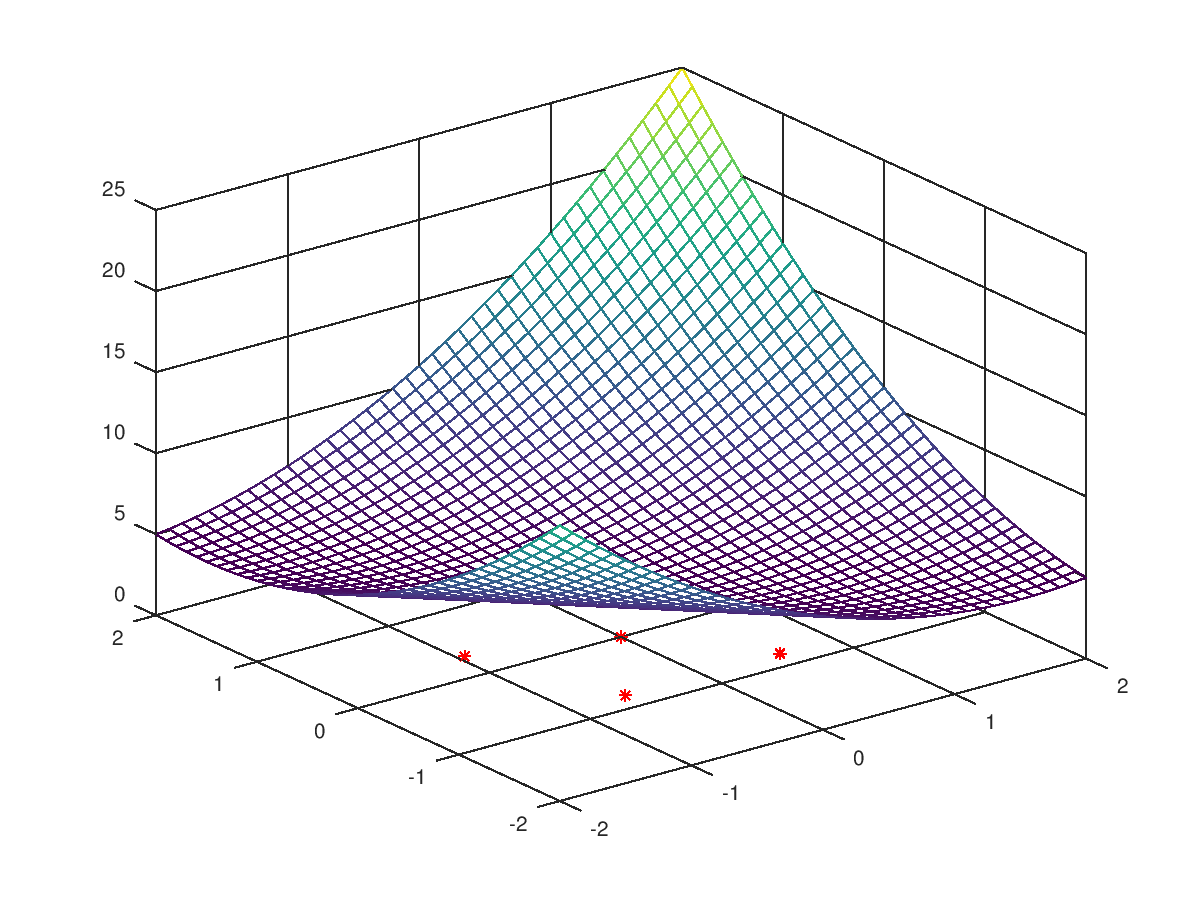
\includegraphics[width=200px]{images/poised_good.png}
    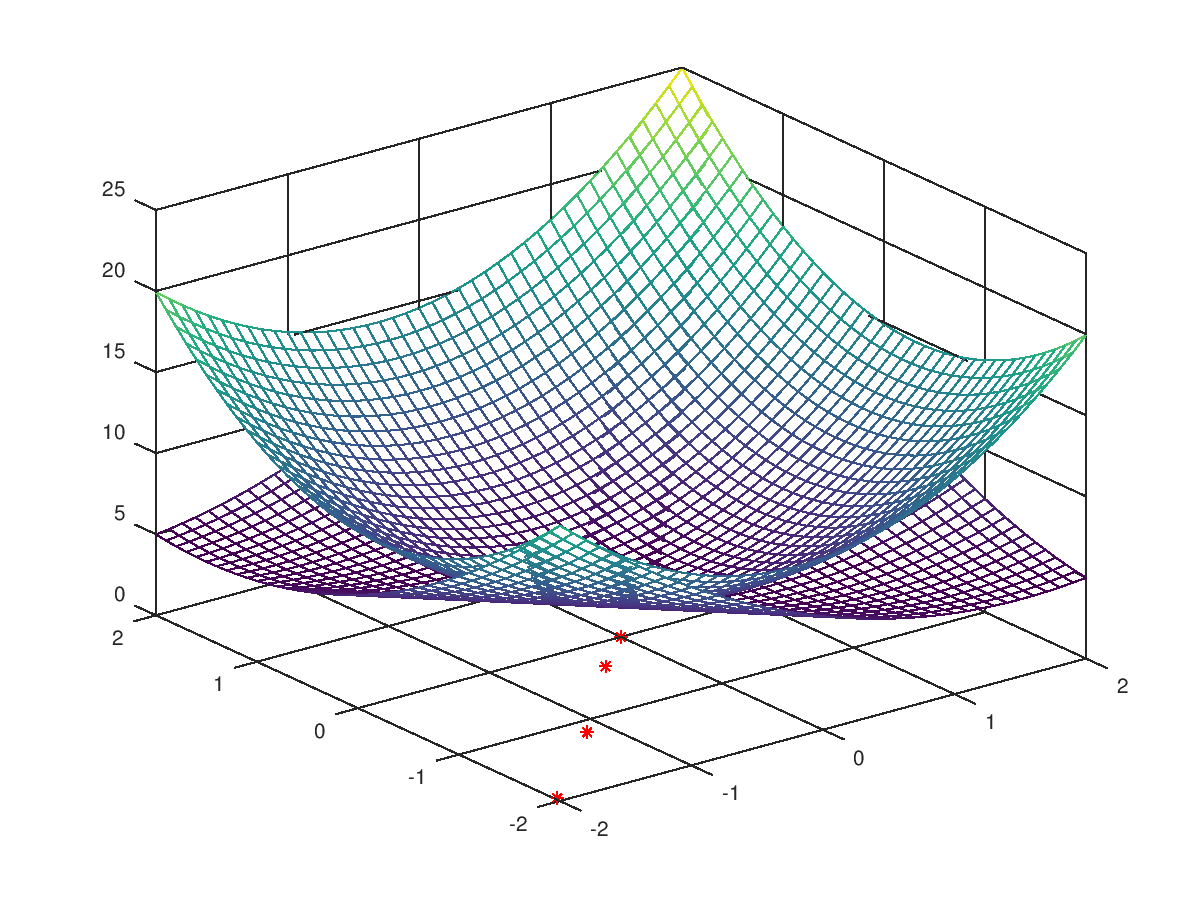
\includegraphics[width=200px]{images/poised_bad.png}
    \caption{Poised vs Ill poised}
    \label{pvip}
\end{figure}


A more detailed discussion can be found in \cite{doi:10.1080/10556780802409296}, but a step to ensure geometry is required for convergence analysis although it may come at the expense of adding more function evaluations.

\paragraph{Geometry Ensuring Algorithms}

Sample points are chosen by a geometry ensuring algorithm.
At any given time, the algorithm has evaluated 0 or more sample points.
Initially, only the starting point $x_0$ is evaluated, so that points must be added.
Evaluated points should be reused when possible, but the algorithm may have to replace some points that are no longer well poised when other new points are selected.
We call the algorithm that adds points, replacing where necessary, the model improvement algorithm.
One classic such algorithm is presented in \cite{DUMMY:intro_book}.

The idea behind this algorithm is to perform an LU factorization with partial pivoting on the Vandermonde matrix.
As we have seen, this computes the basis for the Lagrange polynomials corresponding to $Y$.
However, when this LU factorization encounters a small pivot, the point corresponding to that row is replaced, improving the condition number of the Vandermonde matrix.

In practice, we first shift the sample set $Y$ by subtracting the current iterate and dividing by the trust region radius:
\begin{align}
\bar{Y} = [0, \frac{y^1 - y^0}{\Delta}, \ldots, \frac{y^p - y^0}{\Delta}]
\end{align}

At times, the algorithm will not have all $p+1$ points.
This can be because it is only given one point during initialization, or because points not within the trust region are removed.
Because the model improving algorithm requires all $p+1$ points, we initialize $y^i = y^0$ for any $0 < i \le p$ corresponding to a missing point.
We choose a threshold $0 < \ximin < 1$, and follow \cref{model_improving_algorithm}:

\begin{algorithm}[H]
    \caption{Model Improvement Algorithm}
    \label{model_improving_algorithm}
    \begin{itemize}
        \item[\textbf{Step 0}] \textbf{(Initialization)} \\
            Initialize $i=1$.
            Given a non-empty set $Y$ of user provided points, if $Y$ does not contain $p+1$ points, repeat one of the other points. 
            Construct the Vandermonde matrix $V_{i,j} = \phi_j(\frac 1 {\Delta}(y^i - y^0))$, initialize constant $\ximin > 0$.
        \item[\textbf{Step 1}] \textbf{(Pivot)} \\
            Swap row $i$ with row $i_{\max} = \arg \max_{j|j\ge i} V_{j,i} $
        
        \item[\textbf{Step 2}] \textbf{(Check threshold)} \begin{itemize}
                \item[] If $|V_{i,i}| < \ximin$ then select \label{next_point} $ \hat y = \argmax_{t | \|t\|\le 1} |\phi_i(t)|$.
                \item[] Replace row $i$ with $V_{i, j} \gets \phi_j(\hat y)$.
            \end{itemize}
        
        \item[\textbf{Step 3}] \textbf{(LU)} \begin{itemize}
                \item[] Set $V_i \gets \frac{1}{V_{i,i}} V_i$
                \item[] Set $V_{\bullet j} \gets V_{\bullet j} - V_{i,j} V_{\bullet j} \forall j=i \ldots p$
            \end{itemize}
            Set $i \gets i+1$
            Go to step 1 unless $i = p$
    \end{itemize}
\end{algorithm}
% 
% \paragraph{Proximity}
% 
% Proximity refers to the trust region radius.
% The trust region must go to zero if we are to be sure we have reached a critical point.
% In general, the smaller the trust region, the closer to linear or quadratic the original function will look.
% This is because the model's error term is proportional to the trust region radius.
% 
% In classical trust region algorithms, there is no need for the trust region radius to go to zero.
% Therefore, extra care must be taken to ensure this while modifying such algorithms.


% \begin{algorithmic}
% \If{$\rho < \gamma_1$}
%     \State $\iteratekpone \gets \iteratek$ (reject)
%     \State $\Delta_{k+1} \gets \omega_{\text{dec}} \Delta_k$
% \ElsIf{$\gamma_1 \le \rho \le \gamma_2$}
%     \State $\iteratekpone\gets \gets \iteratek + \trialk$ (accept)
%     \State $\Delta_{k+1} \gets \omega_{\text{dec}} \Delta_k$
% \ElsIf {$\rho > \gamma_2$}
%     \State $\iteratekpone \gets \iteratek + \trialk$ (accept)
%     \If
%         \State $\Delta_{k+1} \gets \omega_{\text{dec}} \Delta_k$
%     \Else
%         \State $\Delta_{k+1} \gets \omega_{\text{inc}} \Delta_k$
%     \EndIf
% \EndIf
% \end{algorithmic}


\subsection{Algorithm Components}




We will discuss several building blocks of the algorithm before going into the algorithm's detail.

\subsubsection{Assessing Model Accuracy and Radius Management}

Each iteration that evaluates a trial point must also test the accuracy of the model functions.
To test the accuracy, we calculate a quantity
\begin{equation}
\label{rho}
\rho_k = \frac{f(\iteratek) - f(\iteratek+\trialk)}{\modelk(\iteratek) - \modelk(\iteratek+\trialk)}
\end{equation}
which measures the actual improvement over the predicted improvement.
A small $\rho_k$ implies the model functions are not sufficiently accurate.
Values of $\rho_k$ close to $1$ imply that the model accurately predicted the new objective value.
A large $\rho_k$ implies progress minimizing the objective although the model was not accurate.
This has been widely used within trust region frameworks such as \cite{Conn:2000:TM:357813} and within a derivative free context \cite{DUMMY:intro_book}.
The user supplies fixed constants $0 < \gammasm \le \gammabi \le 1$ as thresholds on $\rho_k$ and $0 < \omega_{\text{dec}} < 1 \le \omega_{\text{inc}}$ as decrement or increment factors to determine the trust region update policy.
The update policy frequently follows Step 4 within algorithm \cref{unconstrained_dfo} repeated within \cref{trust_region_update} for ease.

\begin{algorithm}[H]
    \caption{Trust Region Update Policy}
    \label{trust_region_update}
    \begin{itemize}
        \item[\textbf{Step 4}] \textbf{(Test for improvement)} \\
            Compute $\rho_k$ with \cref{rho} \begin{itemize}
                \item[] If $\rho_k < \gammasm$ then set $\iteratekpone \gets \iteratek$ (reject) and $\Delta_{k+1} \gets \omegadec\Delta_{k}$
                \item[] If $\rho_k \ge \gammasm$ and $\rho < \gammabi$ then set $\iteratekpone\gets\iteratek+\trialk$ (accept) and $\Delta_{k+1} \gets \omegadec\Delta_{k}$
                \item[] If $\rho_k \ge \gammabi$ and $\|\trialk\| = \Delta_{k}$ then set $\iteratekpone=\iteratek+\trialk$ (accept) and $\Delta_{k+1} \gets \omegainc\Delta_{k}$
                % and either increase the radius or decrease if $\nabla \modelk(\iteratek)$ is small
            \end{itemize}
            $k \gets k+1$ and go to Step 1.
    \end{itemize}
\end{algorithm}




\subsubsection{Criticality Measure}

In order to define stopping criteria for the algorithm, we introduce a criticality measure $\chi$ which goes to zero as the iterates approach a first order critical point.
When the criticality measure is small, we must also decrease the trust region radius.
Once this has reached a small enough threshold $\tau_{\chi}$ and the trust region is small enough ($\Delta_k < \tau_{\Delta}$), we can terminate the algorithm.
For now, our algorithm is designed to work with convex constraints, so we employ a classic criticality measure discussed in \cite{ConnGoulToin00} of

\[
\chik = \|\iteratek - \text{Proj}_{\feasiblek}(\iteratek- \nabla \modelk(\iteratek))\|
\]
where $\feasiblek$ denotes the feasible region: $\feasiblek = \{x \in X | \modelconstrainti(x) \le 0 \quad \forall i \in \mathcal I \wedge c_i(x) = 0 \quad \forall i \in \mathcal E \}$.
This criticality measure measures how far the current is from satisfying the first order optimality conditions for $\iteratek$ to be a constrained minimum of $\modelk$.
When $ \lim_{k\to\infty} \chik = 0$, $\lim_{k\to\infty}\Delta_k = 0$, and $\lim_{k\to\infty}\iteratek = x^{\star}$, then we have that $x^{\star}$ also satisfies the first order optimality conditions of being a constrained minimum of $f$.

%we have $x = \text{Proj}_{\feasiblek}(x - \nabla \modelk(x))$ so that

It can be computed as 
\begin{align}
\label{critical}
\trialk = \min_{s \in \feasiblek} \|\iteratek - \nabla \modelk(\iteratek) - s\|^2 \\
\chik = \|\iteratek - \trialk \|^2 \\
\end{align}

% This remains large while there is feasible search space along a descent direction, but small otherwise or if the gradient goes to zero.

% Namely, when $ \chik(x) = 0$, we have $x = \text{Proj}_{\feasiblek}(x - \nabla \modelk(x))$ so that there is no decent direction along $\nabla \modelk(x)$ as it points away from the feasible region.
% As $\Delta_k$ gets smaller, we also have that $\modelk$ better represents $\nabla f$, so that $\nabla f$ will also either be zero or lie in the iterate's normal cone.

\subsubsection{Sufficient Model Reduction}

To ensure sufficient reduction of the objective's model function during each iteration, we impose the following efficiency condition:
\begin{equation}
\label{efficiency}
\modelk(\iteratek) - \modelk(\iteratek + \trialk) \ge \kappa_f \chi_k \min\{ \frac{\chi_k}{1+\|\nabla^2 \modelk(\iteratek)\|}, \Delta_k, 1 \}
\end{equation}
where $\kappa_f$ is a constant independent of $k$.

This is widely used within trust region frameworks such as \cite{Conejo:2013:GCT:2620806.2621814} and \cite{Conn:2000:TM:357813}.
It can be shown that the \emph{generalized Cauchy point} satisfies this condition.


\subsubsection{Trust Regions}
Our algorithm maintains two trust regions.
The outer trust region is an $L_1$ ball of radius $\Delta_k$ defined by
\begin{equation}
\label{trust_region}
\outertrk = B_{\infty}(\iteratek,\Delta_k) = \{x\in \mathbb R^n | \; {\iteratek}_i - \Delta_k \le x_i \le {\iteratek}_i + \Delta_k \quad \forall 1\le i \le n\}.
\end{equation}

Note that the outer trust region may include infeasible points.
To ensure feasibility of all iterates and sample points, we construct an inner trust region $\innertrk$  satisfying 
$\innertrk \subset \outertrk \cap \feasiblek$ and $\iteratek \in \innertrk$.


We consider two general strategies for constructing $\innertrk$.
\begin{itemize}
\item[1.] Take $\label{redpill} \innertrk = \outertrk \cap \feasiblek$ and ensure model accuracy over a polyhedral domain.
\item[2.] Force $\label{bluepill} \innertrk \subseteq \outertrk \cap \feasiblek$ to have an ellipsoidal shape.
\end{itemize}

The advantage of the second approach is that we can reuse classical methods for ensuring good geometry.
We can choose $\innertrk$ to be ellipsoidal and use efficient algorithms within \cite{DUMMY:intro_book} to satisfy \cref{accuracy}.
However, we must be careful to choose $\innertrk$ to allow sufficient reduction when we solve the trust region subproblem using the inner trust region.


When we use the second approach, have two choices for this trust region subproblem:
\begin{center}
\begin{itemize}
\label{which_trust_region}
\item[2a] $\trialk = \min_{\trialk \in \innertrk \subset \feasiblek} \modelk(\iteratek + \trialk) \label{search_a_little}$
\item[2b] $\trialk = \min_{\trialk \in \outertrk \cap \feasiblek} \modelk(\iteratek + \trialk) \label{search_a_lot}$
\end{itemize}
\end{center}
 
Namely, in 2B with an ellipsoidal inner trust region, we still have to option to select our trial point from the entire $\trialk \in \outertrk \cap \feasiblek$.
To complete 2A $\innertrk = \outertrk \cap \feasiblek$, we need some redefinition of poisedness for polyhedral shapes.
However, since the trust region is larger, it is easier to ensure sufficient reduction.
This strategy also has the drawback that it will force sample points close to the boundary of the feasible region.
If we only model the boundary, this may mean more infeasible evaluation attempts.

The classical methods for ensuring good geometry require an optimization call to the model functions over a sphere.
This is no longer possible in the first approach.
However, the bounds produced over the entire trust region may also be stronger than required as the models will only be used on the feasible region.
This may mean the geometric requirements can be reduced.
Looking again at the ill-poised set in figure \cref{aoip}, the set of nearly collinear sample points actually does appear to be accurate over a smaller trust region.


\begin{figure}[h]
    \centering
    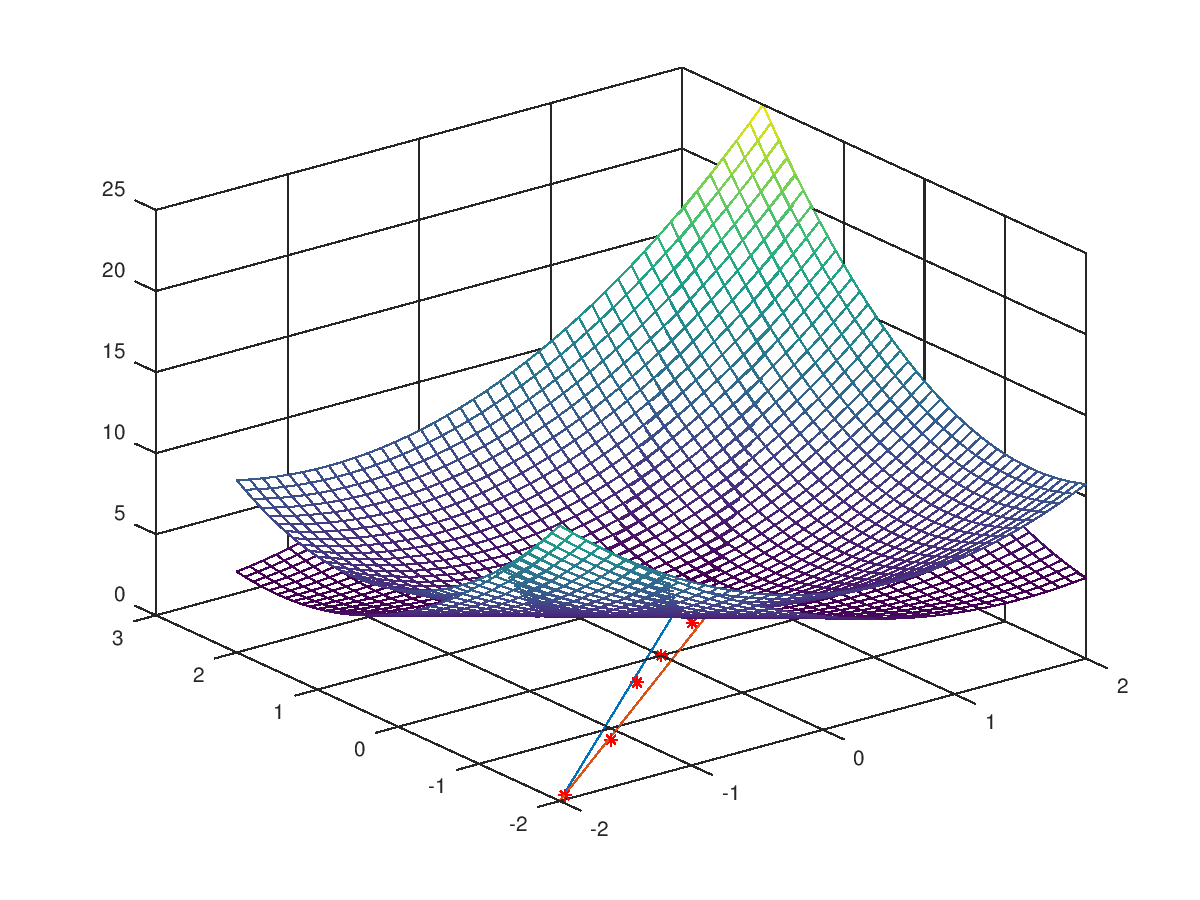
\includegraphics[width=200px]{images/poised_bad_but_good.png}
    \caption{Accurate model over thin trust region from illpoised set}
    \label{aoip}
\end{figure}


Within our algorithm, if $ \outertrk \subseteq \feasiblek$ we can set $\innertrk$ to a sphere.
This saves the computation of $\innertrk$ when it is not needed, as there are no nearby constraints.



\section{Algorithms}

\subsection{Assumptions}
% 
% We assume the following properties.
% 
% \begin{itemize}
% \item The function $f$ is differentiable and its gradient $\nabla f$ is Lipschitz continuous with constant $L > 0$ for all $x \in \domain$.
% \begin{equation}
% \label{A1}
% |f(x_1) - f(x_2)| \le L \|x_1 - x_2\| \quad \forall x_1, x_2 \in \domain
% \end{equation}
% \item \label{A2} The function $f$ is bounded below in $\domain$.
% \begin{equation}
% \label{A2}
% f(x) \ge f_{\text{min}} \quad \forall x \in \domain
% \end{equation}
% 
% \item The Hessians of each model function are uniformly bounded by a constant $\beta \ge 1$ :
% \begin{equation}
% \label{A3}
% \|\nabla^2 \modelk(\iteratek)\| \le \beta - 1 \quad \forall k \ge 0
% \end{equation}
% 
% \end{itemize}

As a first step toward solving a general derivative free problem with partially-quantifiable constraints,
we solve a simpler problem with $\domain = R^n$ and $c(x) = Ax-b$ for some $m\times n$ matrix $A$ and a vector $b\in \mathbb R^m$:

\[ \begin{array}{ccl} \min_{x \in \mathbb R^n} & f(x) \\
& Ax \le b & 
\end{array}
\]
This means that we can let the feasible region be denoted by $\feasible = \{x \in \mathbb R^n | \quad  Ax \le b \}$.
We assume that $A$ has full row rank, and that  $dim(A) = n$.

\subsection{Algorithm Template}

%Although some details depend on the particular choice of $\innertrk$, 
We follow an algorithm template described in \cite{doi:10.1080/10556788.2015.1026968}, where variations of the algorithm have different choices of $\innertrk$ implemented in a \emph{ConstructTrustRegion} subroutine.

% HOW ABOUT JUST MAKE $\eta > 0$?


\begin{algorithm}[H]
    \caption{Always-feasible Constrained Derivative Free Algorithm}
    \label{constrained_dfo}
    \begin{itemize}
        \item[\textbf{Step 0}] \textbf{(Initialization)} \\
            Initialize tolerance constants 
            $\tau_{\xi} > 0$,
            $\tau_{\Delta} > 0$,
            starting point $x^{(0)} \in \domain$,
            initial radius $\Delta_0 > 0$,
            iteration counter $k=0$,
            $0 < \omegadec < 1 \le \omegainc$,
            $0 < \gammasm < \gammabi \le 1$,
            $\alpha > 0$,
            $0 < \Delta_0 < \Delta_{\text{max}} < \frac 1 2 diam(\domain)$,
            $k \gets 1$,
            $0 < \omegadec < 1 \le \omegainc$,
            $0 < \gammasm < \gammabi < 1$.
            
        \item[\textbf{Step 1}] \textbf{(Construct the model)} \\
            $\innertrk\gets $ \Call{ConstructTrustRegion}{$\Delta_k, x^{(k)}$}.
            Ensure that the sample points are poised with respect to $\innertrk$ for \cref{accuracy} by calling algorithm \cref{model_improving_algorithm}.
            Construct $\modelk$ using \cref{reg} to construct $\modelk(x)$.
        
        \item[\textbf{Step 2}] \textbf{(Check stopping criteria)} \\
            Compute $\chi_k$ as in \cref{critical}. \begin{itemize}
                \item[] If $ \chik < \tau_{\xi} $ and $\Delta_k<\tau_{\Delta}$ then terminate.
                \item[] If $ \chik < \tau_{\xi} $ but $\Delta_k\ge\tau_{\Delta}$ then 
                $\Delta_{k+1} \gets \omegadec\Delta_{k}$, 
                $x^{(k+1)} \gets \iteratek$,
                $k \gets k+1$ and go to Step 1.
            \end{itemize}
        
        \item[\textbf{Step 3}] \textbf{(Solve the trust region subproblem)} \\
            Compute $\trialk = \min_{s \in \innertrk} \modelk(\iteratek + \trialk)$.
            \item[] This can also be $\trialk = \min_{s \in \outertrk \cap \feasiblek} \modelk(\iteratek + \trialk)$ depending on the choice made in \cref{which_trust_region}.
            
        \item[\textbf{Step 4}] \textbf{(Test for improvement)} \\
            Evaluate $f(\iteratek + \trialk)$ and evaluate $\rho_k$ as in \cref{rho} \begin{itemize}
                \item[] If $\rho_k < \gammasm$ then $\iteratekpone=\iteratek$ (reject) and $\Delta_{k+1} = \omegadec\Delta_{k}$
                \item[] If $\rho_k \ge \gammasm$ and $\rho < \gammabi$ then $\iteratekpone=\iteratek+\trialk$ (accept), $\Delta_{k+1} = \omegadec\Delta_{k}$
                \item[] If $\rho_k > \gammabi$ then $\iteratekpone=\iteratek+\trialk$ (accept), $\Delta_{k+1} = \omegainc\Delta_{k}$
                % and either increase the radius or decrease if $\nabla \modelk(\iteratek)$ is small
            \end{itemize}
            $k \gets k+1$ and go to Step 1.
    \end{itemize}
\end{algorithm}

 

Much of the work is deferred to the \emph{ConstructTrustRegion} subroutine.
We will describe several different approaches for this subroutine.

% For convergence analysis, \cref{accuracy} must be satisfied by the trust region choice in this method.
%Not all searches for an inner trust region must guarantee this: the algorithm is allowed to try a bounded number of trust regions as long as one is gauranteed to satisfy these conditions.
% In some cases, multiple inner trust regions may be considered before returning the best trust region found.
% An efficient algorithm may first heuristically search for a good trust region if the guaranteed method is expensive.
% This may not involve constructing a model or function evaluations.


\subsection{First Approach: Bumping $\xi$}
One simple approach to handle partially-quantifiable constraints is to maintain the same trust region as the classical algorithm, but avoid letting points fall outside the feasible region within the model improvement algorithm \cref{model_improving_algorithm}.
That is, we add the constraints $\modelconstrainti(x) \le 0 \forall i \in \mathcal{I}$ and $\modelconstrainti(x) = 0 \forall i \in \mathcal{E}$ to the model improvement algorithm while selecting new points.
This constrains the new points to also lie within the current model of the trust region in algorithm \cref{model_improving_algorithm} line \cref{next_point}.
The search space for this optimization problem will be the feasible region intersect the trust region: $\feasiblek \cap \outertrk $.

The problem lies in finding sufficiently poised sample points.
\cref{model_improving_algorithm} uses a parameter $  \ximin $ as a lower bound of the pivot values of the Vandermonde matrix.
This approach could always find a pivot value for any $ \ximin \in (0,1)$ because it optimized over a sphere.
However, when requiring points to live within $ \feasiblek \cap \outertrk $, it can happen that even after replacing a point, we still have not satisfied this bound.
In figure \cref{lspc}, for some values of $  \ximin $, there is no point in $ \feasiblek \cap \outertrk $ that will leave a sufficiently large pivot.

\begin{figure}[h]
    \centering
    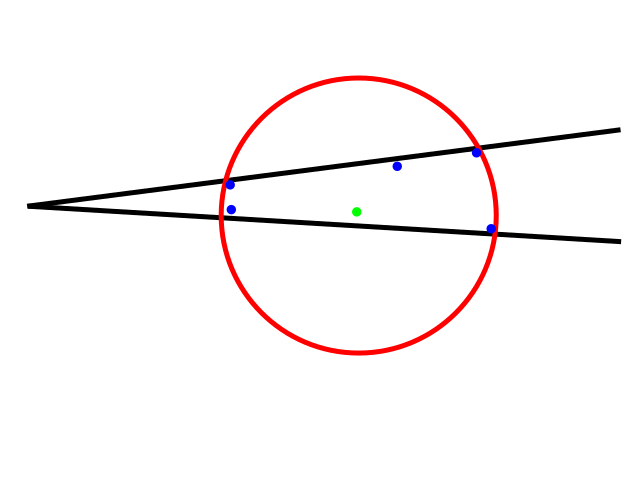
\includegraphics[scale=0.4]{images/bad_lambda.png}
    \caption{Limited sample point choice}
    \label{lspc}
\end{figure}

%As the number of dimensions grows the ratio of volume of the trust region intersect the feasible region to the feasible region can become smaller.

One way to handle this is to introduce a $\xi_{\text{cur}}$ which is allowed to decrease.
(Possibly, until a threshold is reached for maintaining a fixed $\Lambda$.)
If the new point does not improve the geometry of the set significantly, then there is no other point that would do better.
In this case, we cannot do better and simply proceed with our current point.

Alternatively, we can check how much the next point will improve the current pivot, and only replace the existing point if it provides sufficient improvement in the Vandermonde matrix's condition number.



\subsubsection{Requiring Sufficient Model Improvement}

We introduce a constant $0<\delta_{\text{improv}}$ and require that a new point must improve the current pivot by more than $\delta_{\text{improv}}$.
The new modified improvement algorithm is described in \cref{modified_model_improving_algorithm}:


\begin{algorithm}[H]
    \caption{Modified Model Improvement Algorithm}
    \label{modified_model_improving_algorithm}
    \begin{itemize}
        \item[\textbf{Step 0}] \textbf{(Initialization)} \\
            Initialize $i=1$.
            If the current sample set does not have $p$ points, repeat one of the current points. 
            Construct the Vandermonde matrix $V_{i,j} = \phi_j(\frac 1 {\Delta}(y^i - y^0))$,
            $0 < \ximin < \xi_{\text{desired}}$, $0 <\delta_{\text{improv}} < 1$,
            $  \xi_{\text{cur}} = \xi_{\text{desired}}$.
            
        \item[\textbf{Step 1}] \textbf{(Pivot)} \\
            Swap row $i$ with row $i_{\max} = \arg \max_{j|j\ge i} V_{j,i} $
        
        \item[\textbf{Step 2}] \textbf{(Check threshold)} \begin{itemize}
                \item[] If $|V_{i,i}| \ge \xi_{\text{cur}} $ then go to Step 3
                \item[] $ \hat y = \arg\max_{t \in \innertrk \cap X} |\phi_i(t)|$
                \item[] If $\label{impossibly_poised} |\phi_i(\hat y)| < \ximin$ then \textbf{fail}
                \item[] If $\xi_{\text{cur}} - |\phi_i(\hat y)| > \delta_{\text{improv}} \xi_{\text{cur}}$ then replace $V_{i,j}$ with $\phi_j(\hat y)$ and $\xi_{\text{cur}} \gets |\phi_i(\hat y)|$
            \end{itemize}
        
        \item[\textbf{Step 3}] \textbf{(LU)} \begin{itemize}
                \item[] Set $V_i \gets \frac{1}{V_{i,i}} V_i$
                \item[] Set $V_{,j} \gets V_{, j} - V_{i,j} V_{, i} \forall j=i \ldots p$
            \end{itemize}
            $i \gets i+1$
            Go to step 1 unless $i > p$
    \end{itemize}
\end{algorithm}

The \emph{ConstructTrustRegion} subroutine for this approach follows the prototype with $T_{in} = \feasiblek \cap \outertrk $.
As is usual, we may also wish to remove points larger than a certain radius from the current model center.
% If a lower bound $\kappa_{\phi}$ on the maximum value of each polynomial is known ahead of time, then the check on \cref{impossibly_poised} is not needed.
% That is, for a given set of linear constraints and largest trust region radius, it may be possible to calculate $\xi_{\text{min}} \le \kappa_{\phi} \le \max_{V}\max_{j}\max_{i}\|\phi_i(y^j)\|$.

%Another interesting approach we have not investigated is to decrease the size of the sample set when a new point cannot be computed.

%The analysis for this approach may be more difficult.




\subsection{Second Approach: Feasible Trust Regions}

If we adopt the second approach to maintain a feasible inner trust region with a ``nice" shape, we ensure of a stronger version of \cref{accuracy}.
Namely, we will know that 
\[
    \|\modelk(x) - \nabla f(x) \| \le \kappa_g \Delta_{k} \quad \forall x \in \innertrk.
\]
If we also choose to our trial point with \cref{search_a_little}, we have no guarantee of \cref{efficiency}.
However, the model will likely be more accurate over this region.

%If bounds can be shown relating the model error of the inner trust region to the outer trust region, then we will satisfy \cref{accuracy}.
%In this case, classical methods ensure that $\|\nabla f(x^{(k)}) - \nabla m_f(x^{(k)})\| < \Delta_{inner} \le \Delta_k$.

\subsubsection{Circular Trust Region}
The simplest approach to maintaining a feasible trust region is to set the inner trust region radius sufficiently small.
Within the \emph{ConstructTrustRegion} subroutine, this method sets the trust region radius to the distance to the closest constraint:
$\outertrk = B_2(\iteratek, \min\{\Delta_k, \min_{i}\frac{|A_i\iteratek - b_i|}{\|A_i\|} \})$.

In practice, this does not work well as the radius can become too small to allow any progress.

\begin{figure}[h]
    \centering
    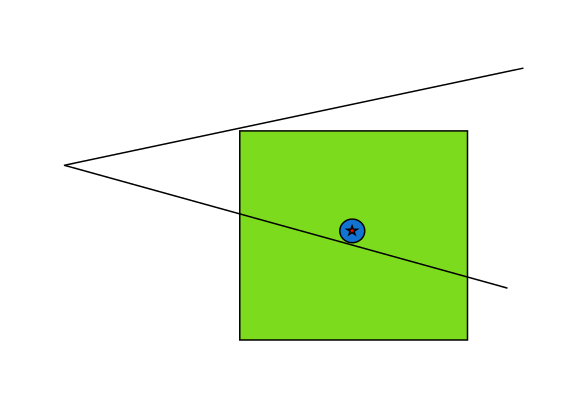
\includegraphics[width=200px]{images/small_circle.png}
    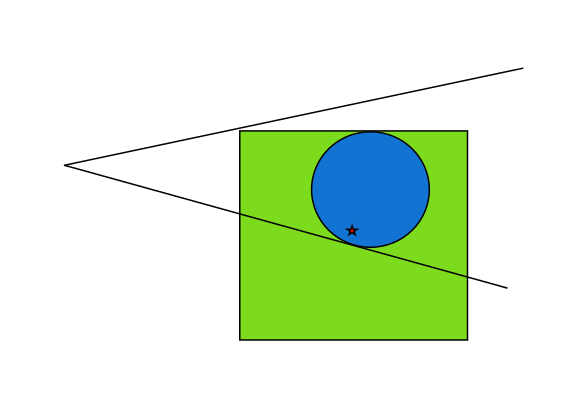
\includegraphics[width=200px]{images/shifted_center.png}
    \caption{When the current iterate is too close to a constraint, the circular trust region becomes too small. Shifting trust region center helps to remedy this. The star is the current iterate, the green is the outer trust region, and blue the inner.}
    \label{options_basis}
\end{figure}

Two general strategies were considered for addressing this issue as illistrated in \cref{options_basis}.
One option is to shift the center of the inner trust region as long as it remains within the outer trust region.
The second option is to elongate the trust region along the nearest constraint as discussed in the next section.
Of course, both of these can be done at the same time.


\subsubsection{Ellipsoids}

In order to address this issue we considered using ellipsoidal trust regions.
Whereas the circle does not allow improvement when the current iterate lies along a constraint, an ellipse elongates along this constraint.
In figure \cref{ellipse_adv}, we have this type of iterate, but by using an ellipse we are still able to search towards the vertex of the feasible region.
\begin{figure}[h]
    \centering
    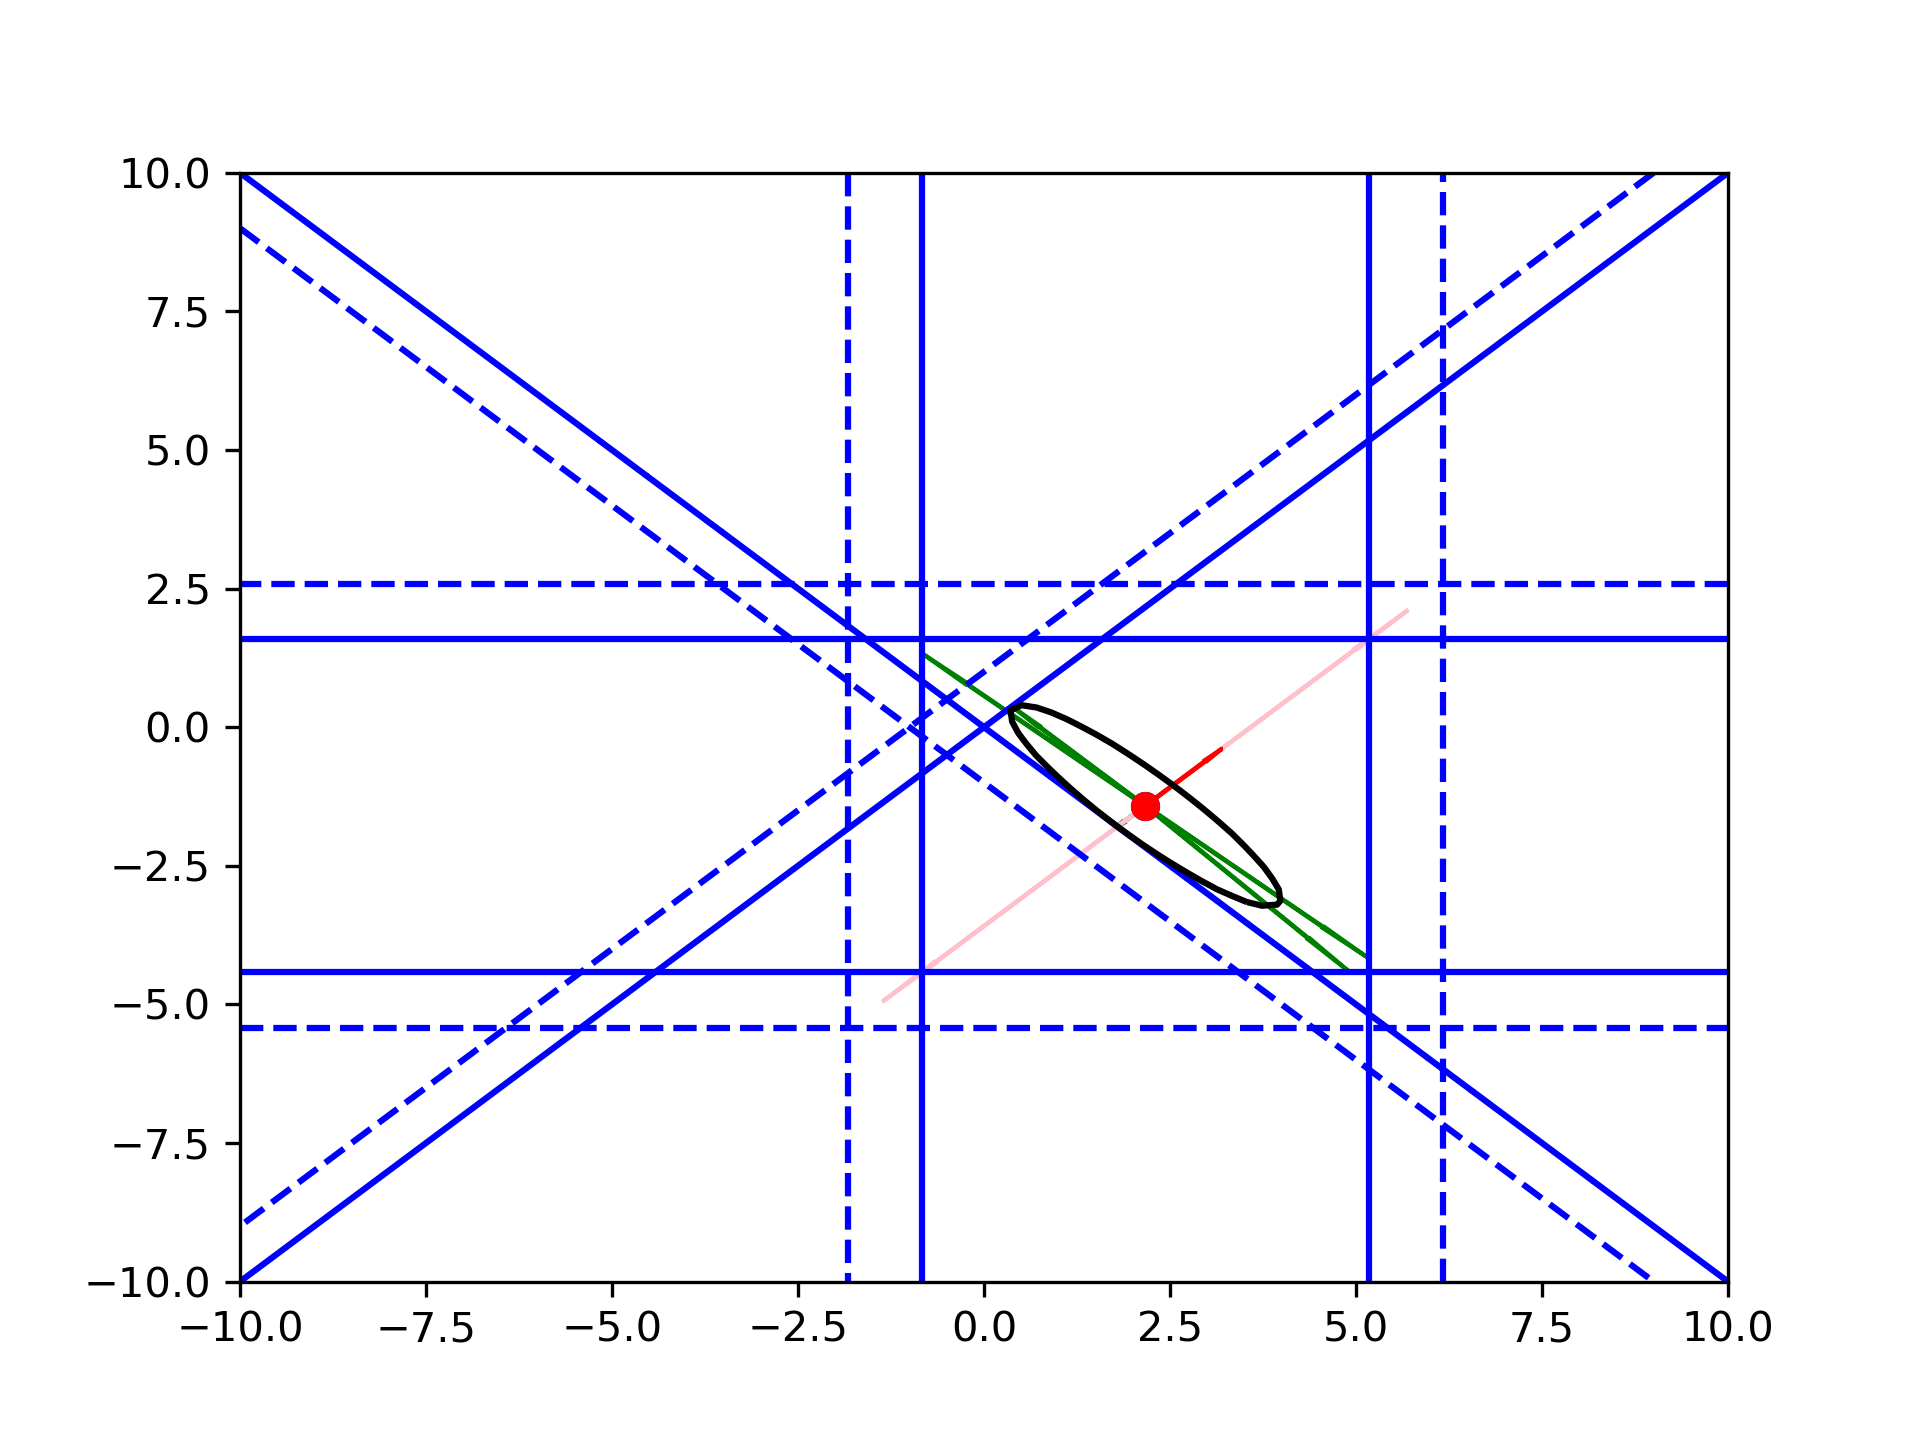
\includegraphics[scale=0.4]{images/advantage_of_ellipse_2.png}
    \caption{A nicer trust region}
    \label{ellipse_adv}
\end{figure}


More specifically, at iteration $k$, we choose a scaling factor $\pi^k$ and solve for an ellipse center $\mu^k$ and positive definite matrix $Q^k$ to define an ellipse
$ \ellipsek = \{x \in \mathbb R^n \| \pi^k - \frac 1 2 (x - \mu^{k})^TQ^{k}(x - \mu^{k}) \ge 0 \}$.
% We then map this back to the origin with the affine transformation $T : \mathbb R^n \to R$, $T(x) = \frac {\sqrt{2}}{\pi^k} L^k(x-\mu^k)$ where $L = cholesky(Q)$.
% This allows us to construct a $\Lambda$-poised set within narrow trust regions.
Of course, the simplest approach is to not change the center of the ellipse, but instead let $\mu^k = x^k$.


\subsubsection{Finding the Maximal $ \ellipsek $ Given $\mu^k$}

\label{ellipse_optimization}

Here, we first solve the problem of finding the maximum-volume ellipse given the center.
Later we perform a search over different centers of the ellipse.
%Because of this, we will first show how to find an ellipse with maximum volume given a fixed center.
We adopt a method similar to \cite{Khachiyan1993}.
For now, we also let $\pi^k = 1$.

Given a polyhedron $P$ defined by an $m \times n$ matrix $A$,
\[
P = \{ x \; | \;  Ax \le b \},
\]
we wish to find the maximum-volume ellipse $E \subset P$ centered at a point $\mu^{k}$ within this polyhedron.

Let $\bar{b} = b - A\mu^{k}$ and $d = x - \mu^{k}$ so that the polyhedron becomes
\[
P = \{ \mu^k + d \; | \;  Ad \le \bar{b} \}
\]
The ellipse can then be centered at zero, and defined by a symmetric positive definite matrix $Q \succ 0$:
\[
E = \{ d \; | \; \frac 1 2 d^T Q d \le 1 \}.
\]
Our goal is to determine $Q$ to maximize the volume of $E$ such that $\mu^{k} + E \subset P$.
Define the auxiliary function 
\[
f(d) = \frac 1 2 d^T Q d
\]
so that 
\[
E = \{ d \; | \; f(d) \le 1 \}.
\]

Because $Q$ is positive definite, $f$ has a unique minimum on each hyper-plane $A_i d = b_i$.
Let this minimum be $d^{(i)} = \argmin_{d\| A_id =\bar{b}_i} f(d)$ for $i=1,\ldots,m$.
By the first order optimality conditions, there exists a $\lambda \in \mathbb R^m$ such that
\[
\nabla f(d^{(i)}) = Q d^{(i)} = \lambda_i A_i \quad \forall 1\le i\le m
\]
\[
\Rightarrow d^{(i)} = \lambda_i Q^{-1}A_i \quad \forall 1\le i\le m
\]
We also know that 
\[
A_i^T d^{(i)} = \bar{b_i}
\]
\[
A_i^T \lambda_i Q^{-1}A_i = \bar{b_i}
\]
\[
\lambda_i = \frac {\bar{b_i}}{A_i^T  Q^{-1}A_i}
\]
so that 
\[
d^{(i)} = \lambda_i Q^{-1}A_i = \frac {\bar{b_i}}{A_i^T  Q^{-1}A_i}  Q^{-1}A_i \quad \forall 1\le i\le m.
\]

Because $E \subset P$, we also know that $f(d^{(i)}) \ge 1$ for each $i$. Thus,
\[
\frac 1 2 (d^{(i)})^{T} Q d^{(i)} \ge 1
\]
\[
\Rightarrow \frac 1 2 (\frac {\bar{b}_i}{A_i^T  Q^{-1}A_i}  Q^{-1}A_i)^{T} Q \frac {\bar{b}_i}{A_i^T  Q^{-1}A_i}  Q^{-1}A_i \ge 1
\]
\[
\Rightarrow \frac 1 2 \frac {1}{A_i^T  Q^{-1}A_i}  \bar{b_i} A_i^T Q^{-1} Q \frac {\bar{b_i}}{A_i^T  Q^{-1}A_i}  Q^{-1}A_i \ge 1
\]
\[
\Rightarrow \frac 1 2 \frac {1}{A_i^T  Q^{-1}A_i}  \frac {\bar{b_i}^2}{A_i^T  Q^{-1}A_i}  A_i^T Q^{-1}A_i \ge 1
\]
\[
\Rightarrow \frac 1 2  \frac {\bar{b_i}^2}{A_i^T  Q^{-1}A_i} \ge 1
\]
\[
\Rightarrow \frac 1 2 \bar{b_i}^2\ge A_i^T  Q^{-1}A_i
\]
\[
\Rightarrow A_i^T  Q^{-1}A_i \le \frac 1 2 \bar{b_i}^2
\]

Because the volume of the ellipsoid is proportional to the determinant of $Q^{-1}$, the maximal ellipse is defined by

\[
\sup_{Q \succeq 0} \det(Q^{-1})
\]
\[
s.t. \quad A_i^T Q^{-1} A_i \le \frac 1 2 \bar{b_i}^2
\]


This problem includes a maximization of a determinant.
In order to ensure that the trust region goes to zero, we must also ensure that the maximum eigenvalue of the matrix is bounded.
Thus, for some bound $M^k$ we define $Q^k$ as

\begin{center}
\begin{align}
\label{ellipse_1}
Q^k = V(\mu^k) = \sup_{Q \succ 0} & \det(Q^{-1}) & \\
  & {A^k}_i^T Q^{-1} {A^k}_i \ge \frac 1 2 (b^k - A^k\mu^{k})^T(b^k - A^k \mu^{k}) & \\
  & eig(Q)_i \le M^k & \forall i \in \mathcal I \cup \mathcal E \\
  & \pi^k - \frac 1 2 (x^k - \mu^{k})^TQ^{k}(x^k - \mu^{k}) \ge 0
\end{align}
\end{center}

if we wish to include the original point explicitly.
This gives rise to the trust region sub problem of

$$\innertrk = \{x \in \mathbb | 1 - \frac 1 {2s^k} (x - \mu^{k})^T Q (x - \mu^{k}) \ge 0\} $$
$$\trialk = \max \{1, \frac 1 {2} (\iteratek - \mu^{k})^T Q^k (\iteratek - \mu^{k})^T \}$$


\subsubsection{Ellipse Choices}

There are a number of issues to be solved to define this ellipse:
\begin{itemize}
\item How do we ensure that $\iteratek \in \ellipsek$?
\item How do we choose the center of the ellipse $\mu^k$?
\item How do we choose $Q^{k}$ to make the  ellipse as large as possible while ensuring that $ \ellipsek \subset \outertrk \cap \feasiblek$?
\end{itemize}

We have implemented a few ways of ensuring the current iterate is within the trust region, $\iteratek \in \ellipsek$.
If we do not include the current iterate within the interior of $\innertrk$, we likely lose sufficient reduction.
This can be done by either expanding the radius of the ellipse, or by including the original point as a constraint for the ellipse problem.

%IMAGES GO HERE

In order to include the original point as a constraint, we add a constraint to the definition of the ellipse of the following form:
$$ \pi^k - \frac 1 2 (x^k - \mu^{k})^TQ^{k}(x^k - \mu^{k}) \ge 0. $$
Constraints of this nature make the optimization problem of finding the ellipse much more expensive.
This is because the optimization problem we construct to find $Q^k$ solves for ${Q^k}^{-1}$, so that adding this constraint is a constraint on the inverse of our decision variable ${Q^{k}}^{-1}$.


The alternative is to scale $Q$ by a constant.
To do this, we use the scaling factor $\pi^k$ by defining it to be

$$\pi^k = \max \{1, \frac 1 {2} (x^{k} - \mu^{k})^T Q^k (x^{k} - \mu^{k})^T \}$$

and let the ellipse be:
$$E_k = \{x \in \mathbb | 1 - \frac 1 {2\pi^k} (x - \mu^{k})^T Q (x - \mu^{k}) \ge 0\} $$
However, this means that we do not ensure $E_k \subset F_k$ so that the trust region subproblem must contain constraints for both the ellipse and the feasible region: $\innertrk = \ellipsek \cap \domain$.

The are several concerns to be considered while defining the ellipse.
The major concern is that we can accidentally define $\ellipsek$ in such a way that it limits travel along a decent direction.
%We also want consecutive ellipse to share volume, in order to avoid evaluating as many points as possible.
%(So far, we have been re-evaluating the set of trial points each iteration.)


Also, unless we include points outside the ellipse, we cannot find a second order solution because the ellipse can only be tangent to the constraint.
In \cref{fbns}, the red line represents a path in the feasible region that is always decreasing.
However, if the trust regions decrease without intersecting this path, the algorithm will not be aware of this descent path.
However, scaling the trust region to the outer green radius may allow the algorithm to ensure global convergence to second order critical points.

\begin{figure}[h]
    \centering
    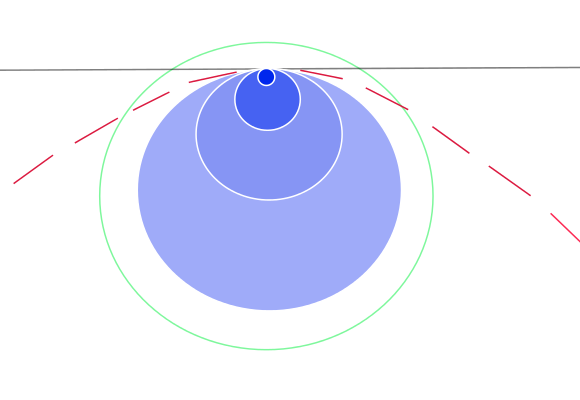
\includegraphics[width=200px]{images/second_order_critical_point.png}
    \caption{Potential issue with a second order critical point}
    \label{fbns}
\end{figure}



Finally, we have the problem of computing the ellipse once given a suitable definition.
In order to provide the most search space available within the trust region subproblem, we maximize the volume of the ellipse.

\subsection{Searches for the Center}

We consider several different approaches for determining the trust region center $\mu^k$.
In this case, our \emph{ConstructTrustRegion} subroutine searches over multiple centers of the ellipse, however it may not need to construct the model functions for each until it has found a desirable ellipsoid.

Given a huristic $H : \innertrk \to \Theta$, where $\Theta$ is a set of comparable elements, the \emph{ConstructTrustRegion} routine follows the following template:

\begin{algorithm}[H]
    \caption{Heuristic Search}
    \label{heuristic_search}
    \begin{itemize}
        \item[] \textbf{Initialization} Initialize $T_{\text{best}} = \emptyset$, $\theta_{\text{best}} = H(T_{\text{best}})$
            
        \item[] \textbf{For all $\mu \in$ search space do:} \begin{itemize}
                \item[] $T_{\text{trial}} \gets \arg\max_{E_k \text{centered at} \mu} \text{Vol}(E_k)$
                \item[] $\theta_{\text{trial}} = H(T_{\text{trial}})$
                \item[] If $\theta_{\text{trial}} \le \theta_{\text{best}}$ then continue
                \item[] $T_{\text{best}} = T_{\text{trial}}$
                \item[] $\theta_{\text{best}} = \theta_{\text{trial}}$
            \end{itemize}
    \end{itemize}
\end{algorithm}

In most cases, we have simply used the heurstic $H(E_k) \to \text{Vol}(E_k)$.

\subsubsection{Search Everything}

One approach is to search all possible centers within $ \feasiblek \cap \outertrk $.
That is, we add the constraints directly to the trust region subproblem by modifying \cref{ellipse_1}:
$$\mu^k = \sup_{\mu \in \feasiblek \cap \outertrk} V(\mu)$$
%The search within the \emph{ConstructTrustRegion} is allowed to go anywhere within $ \feasiblek \cap \outertrk$.
This has the advantage that it captures much of the feasible region.
However, one problem with this search is that it can force the trust region away from the desired direction.
Notice that in \cref{ellipse_runs_away}, although the ellipse found has larger volume than before being shifted, this ellipse contains points further from corner containing the minimizer.

\begin{figure}[h]
    \centering
    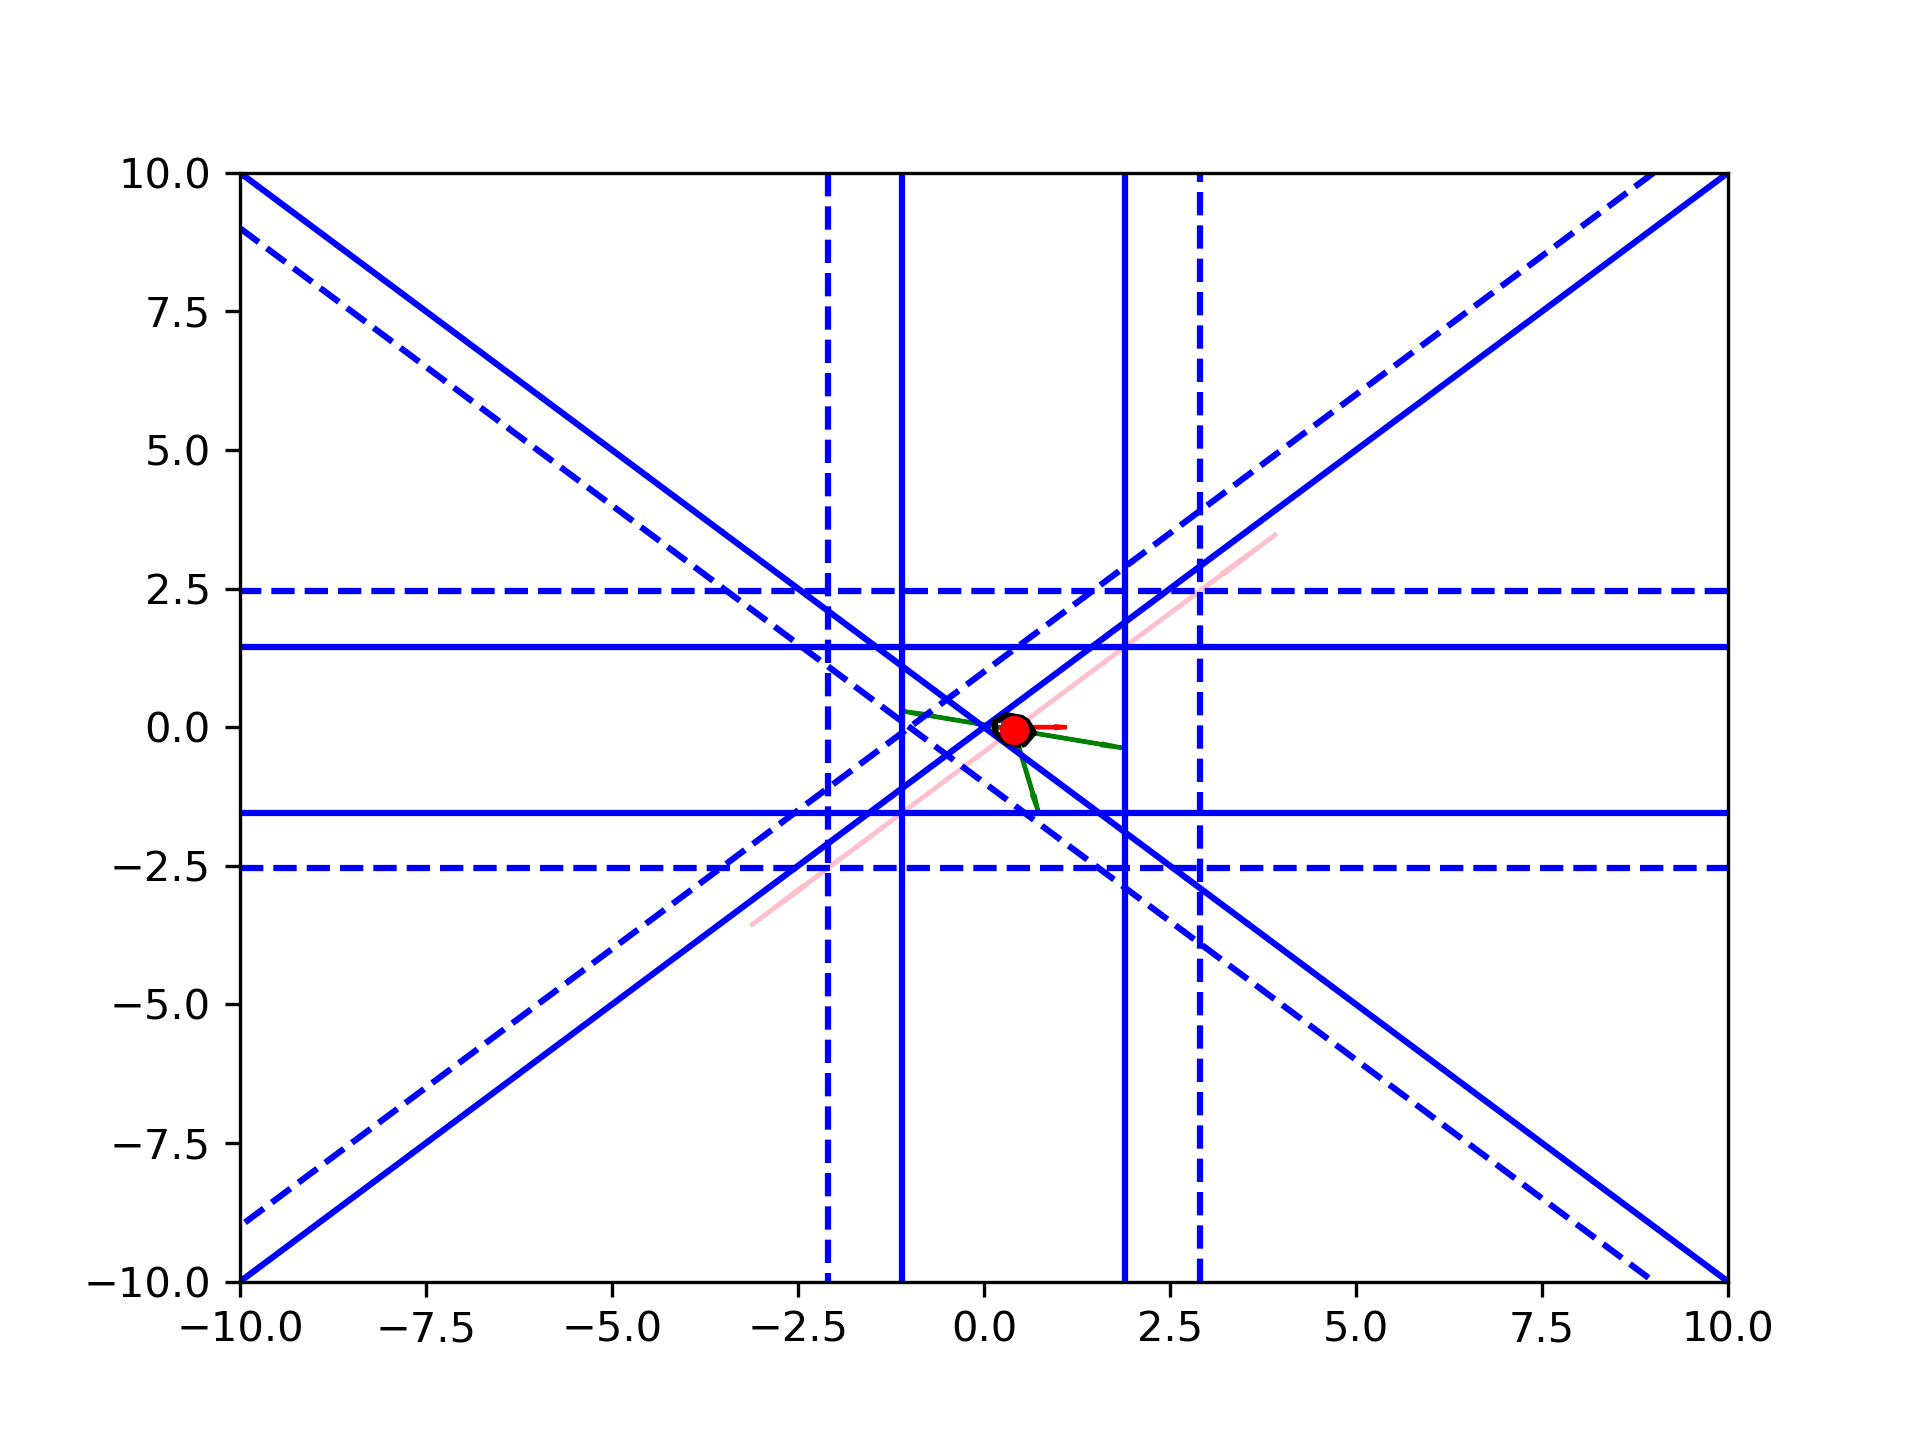
\includegraphics[scale=0.4]{images/everything_runs_1.png}
    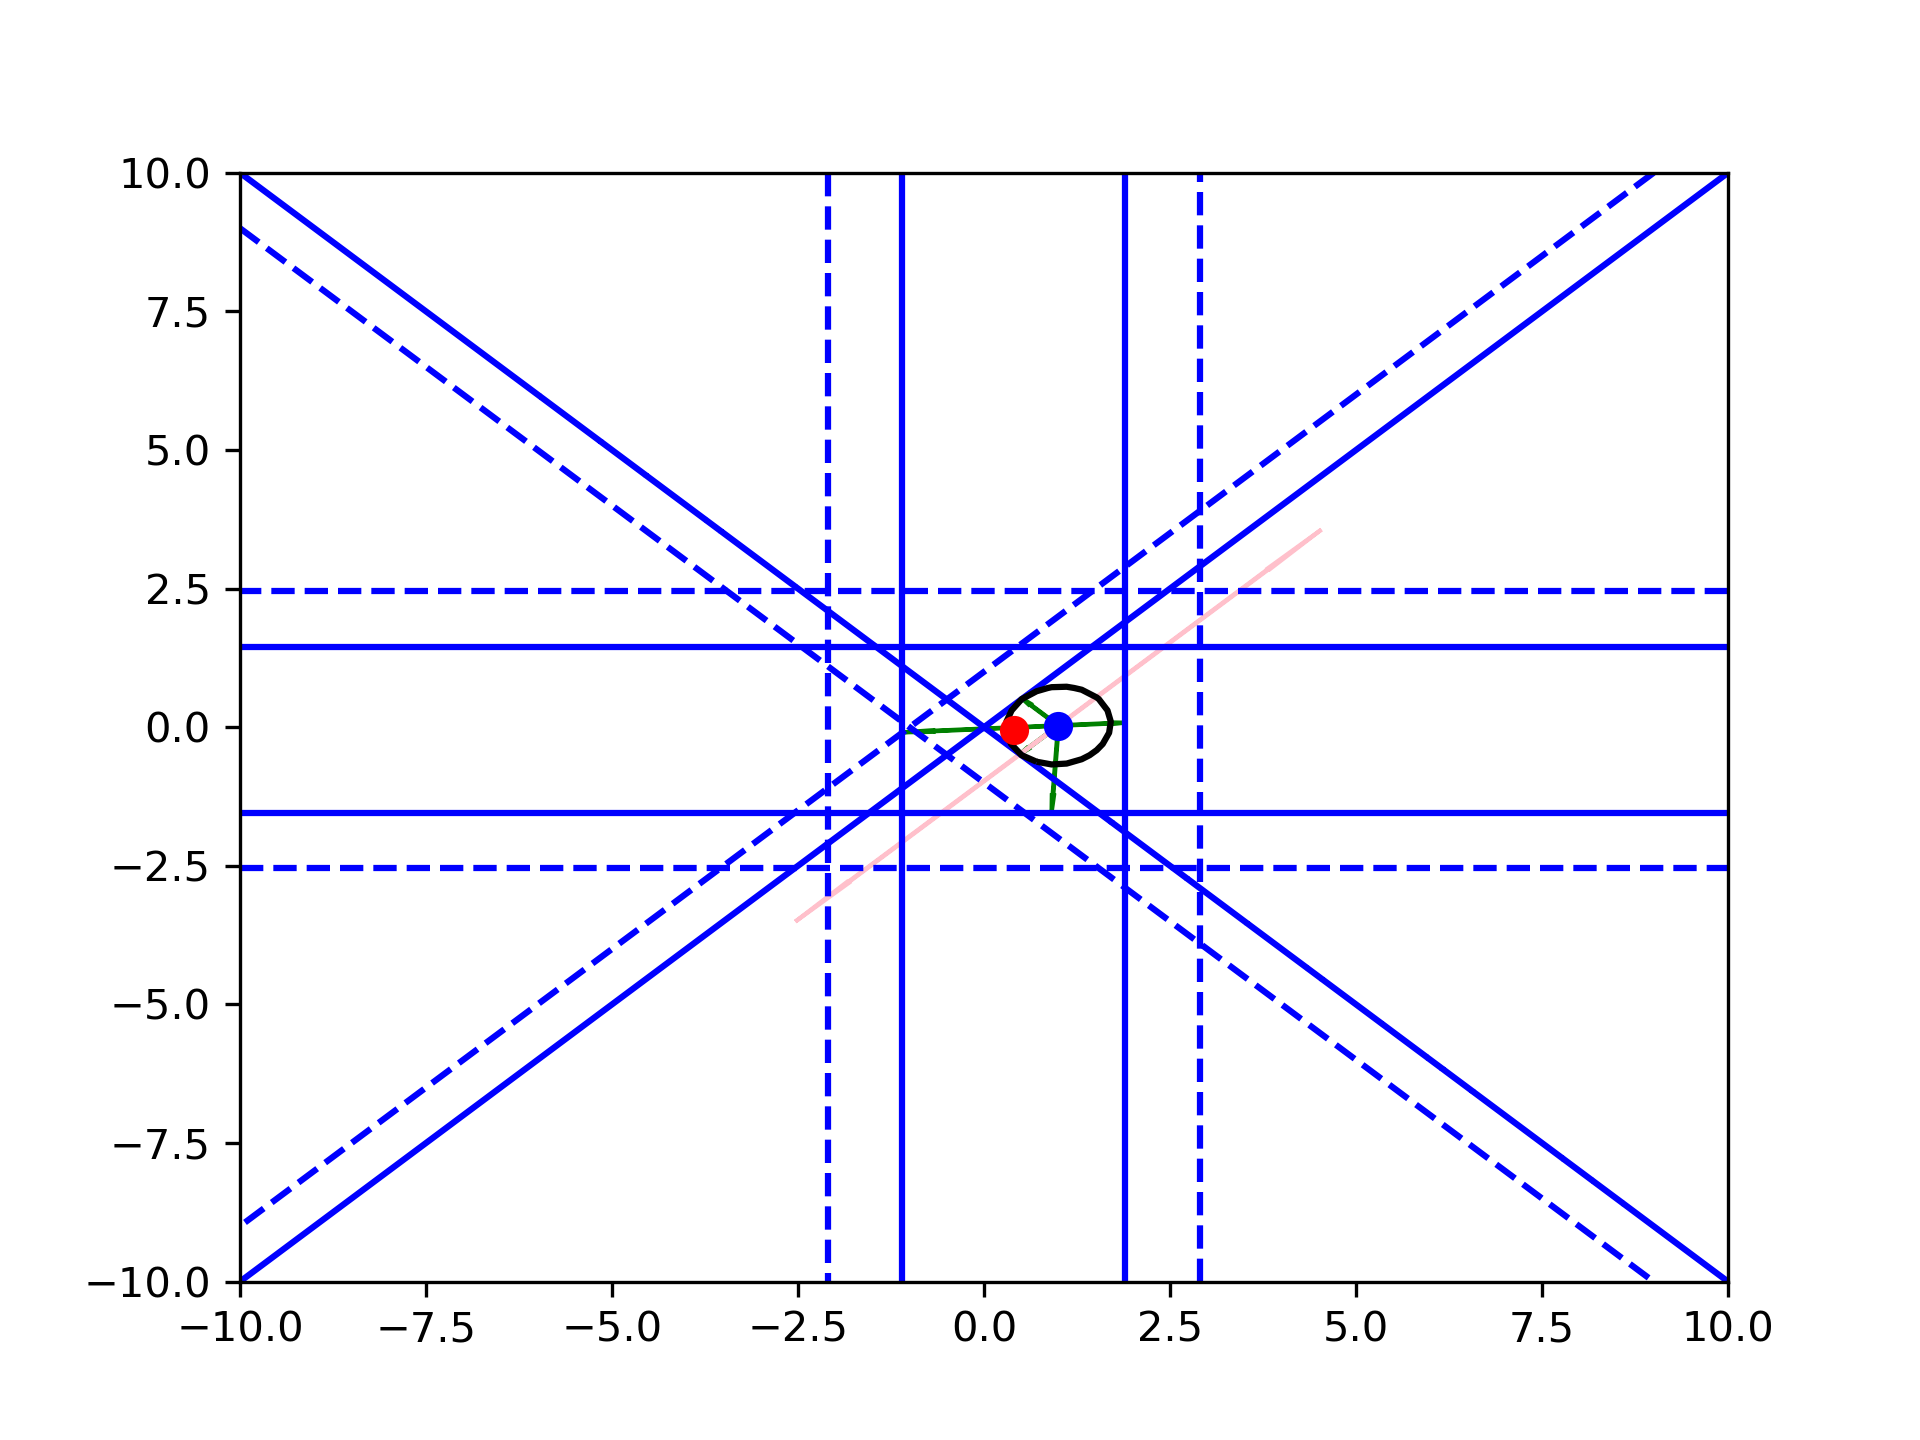
\includegraphics[scale=0.4]{images/everything_runs_2.png}
    \caption{Searching $\feasiblek$}
    \label{ellipse_runs_away}
\end{figure}


One attempt to fix this problem is by limiting the search direction for the center of the ellipse.


\subsubsection{Line Searches}
Although $\modelk$'s minimizer over $\outertrk$  can appear anywhere, there are some reasons for expecting it to be at a ``vertex."
If it lies on the interior, there is little need for using constrained approaches once near the solution.

The ellipse with maximum volume, however, tends to lead $\innertrk$ away from vertices.
One way of trying to ensure a feasible direction towards a vertex, while still allowing a larger volume ellipse, is by limiting the search for the new center to lie on line segments starting at the current iterate $\iteratek$.

For example, our first attempt was to simply search a line directed orthogonally away from the closest constraint.
This has obvious problems as shown in \cref{first_line_search}, as we should avoid letting the new center get closer to another constraint:

\begin{figure}[h]
    \centering
    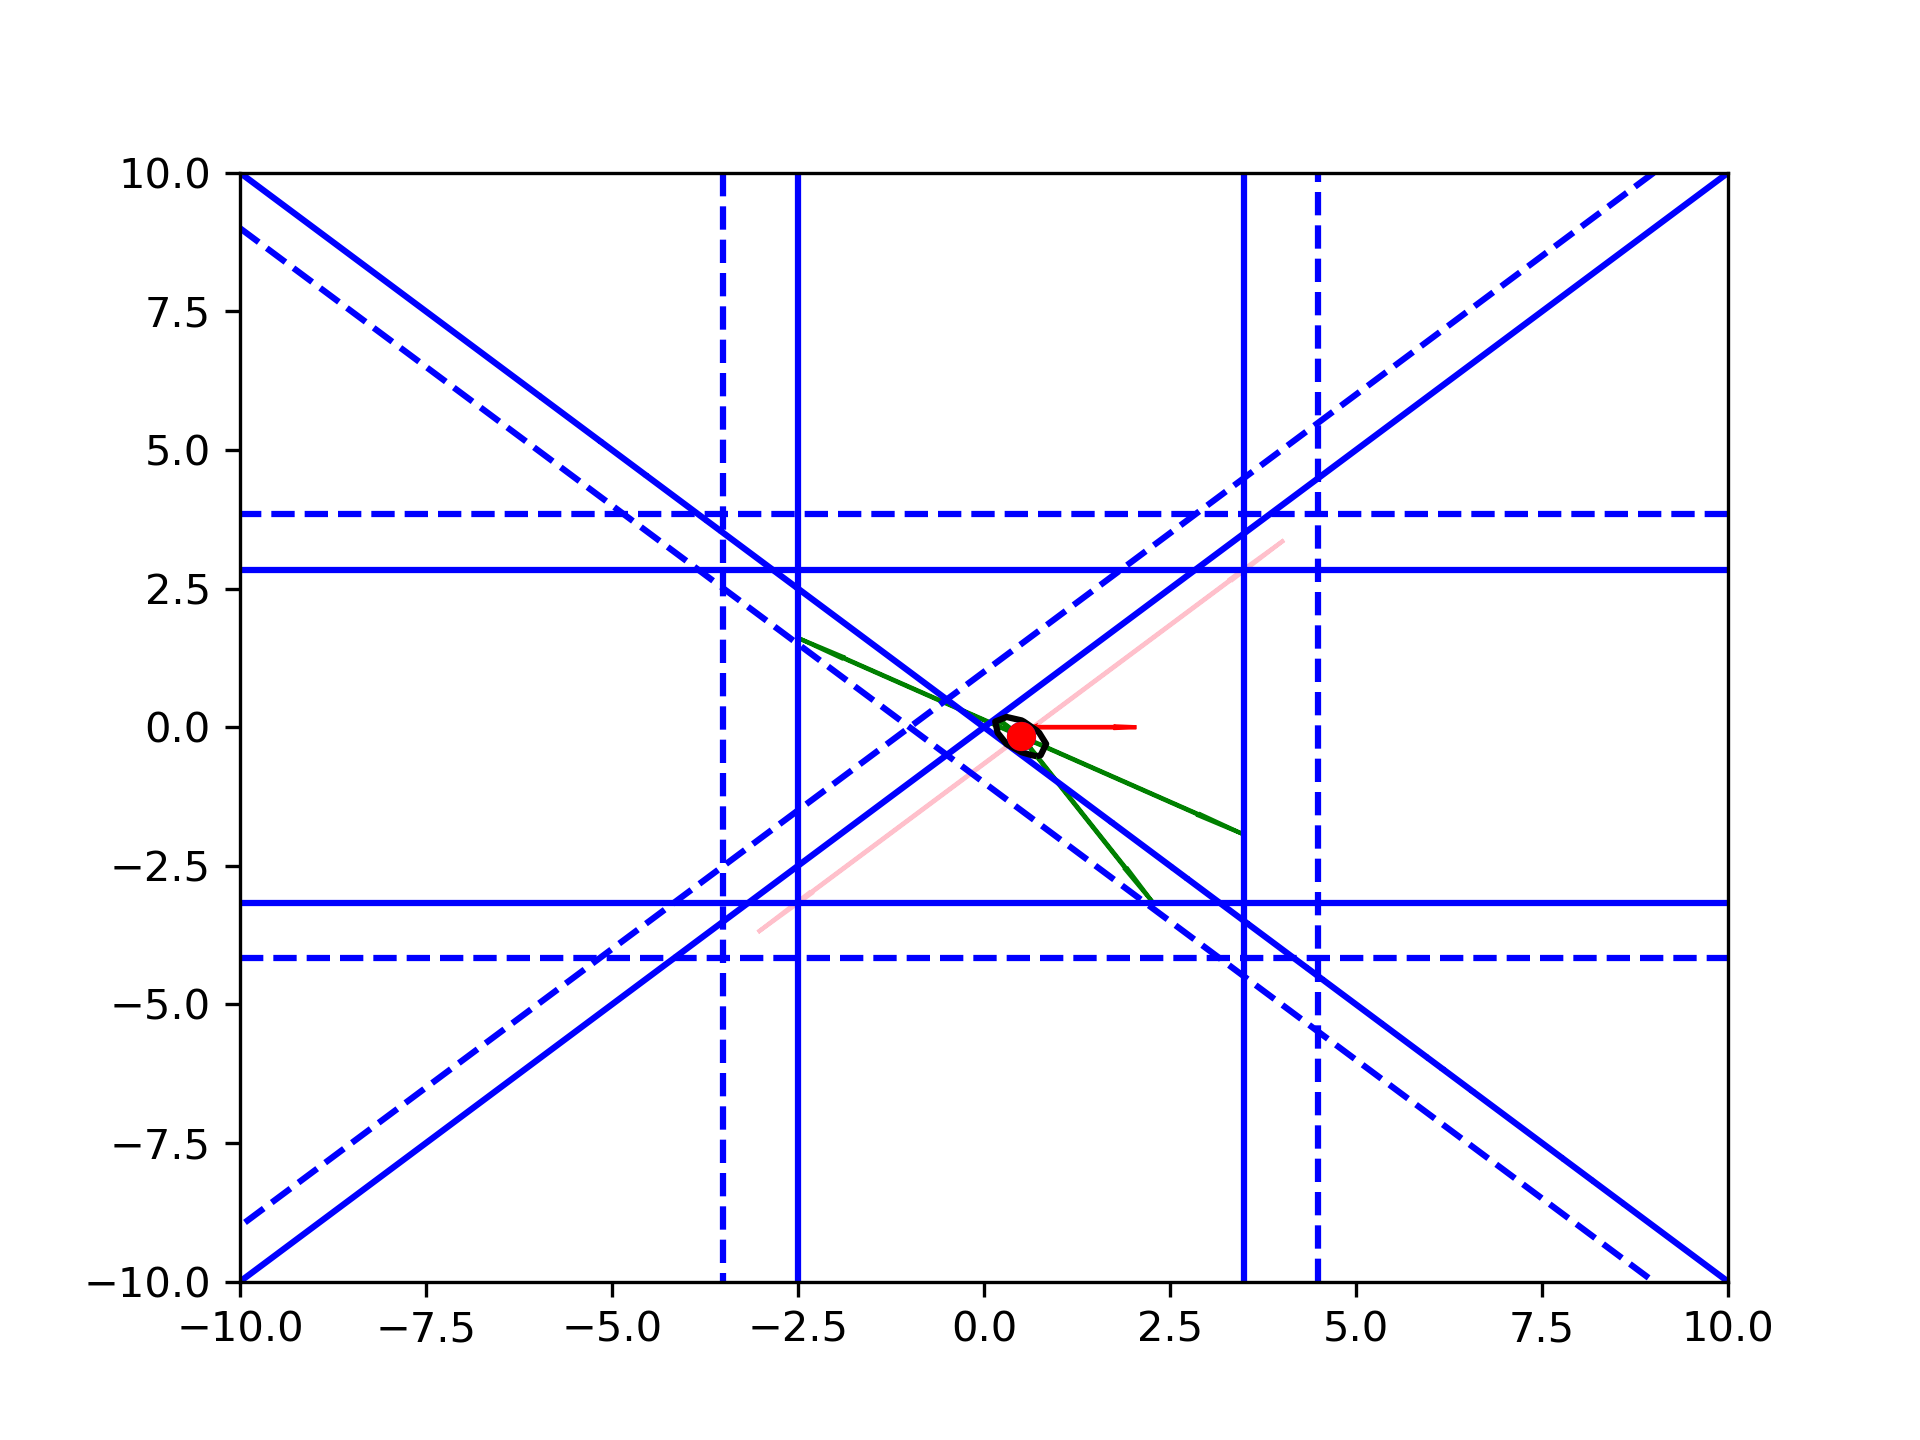
\includegraphics[scale=0.4]{images/line_1.png}
    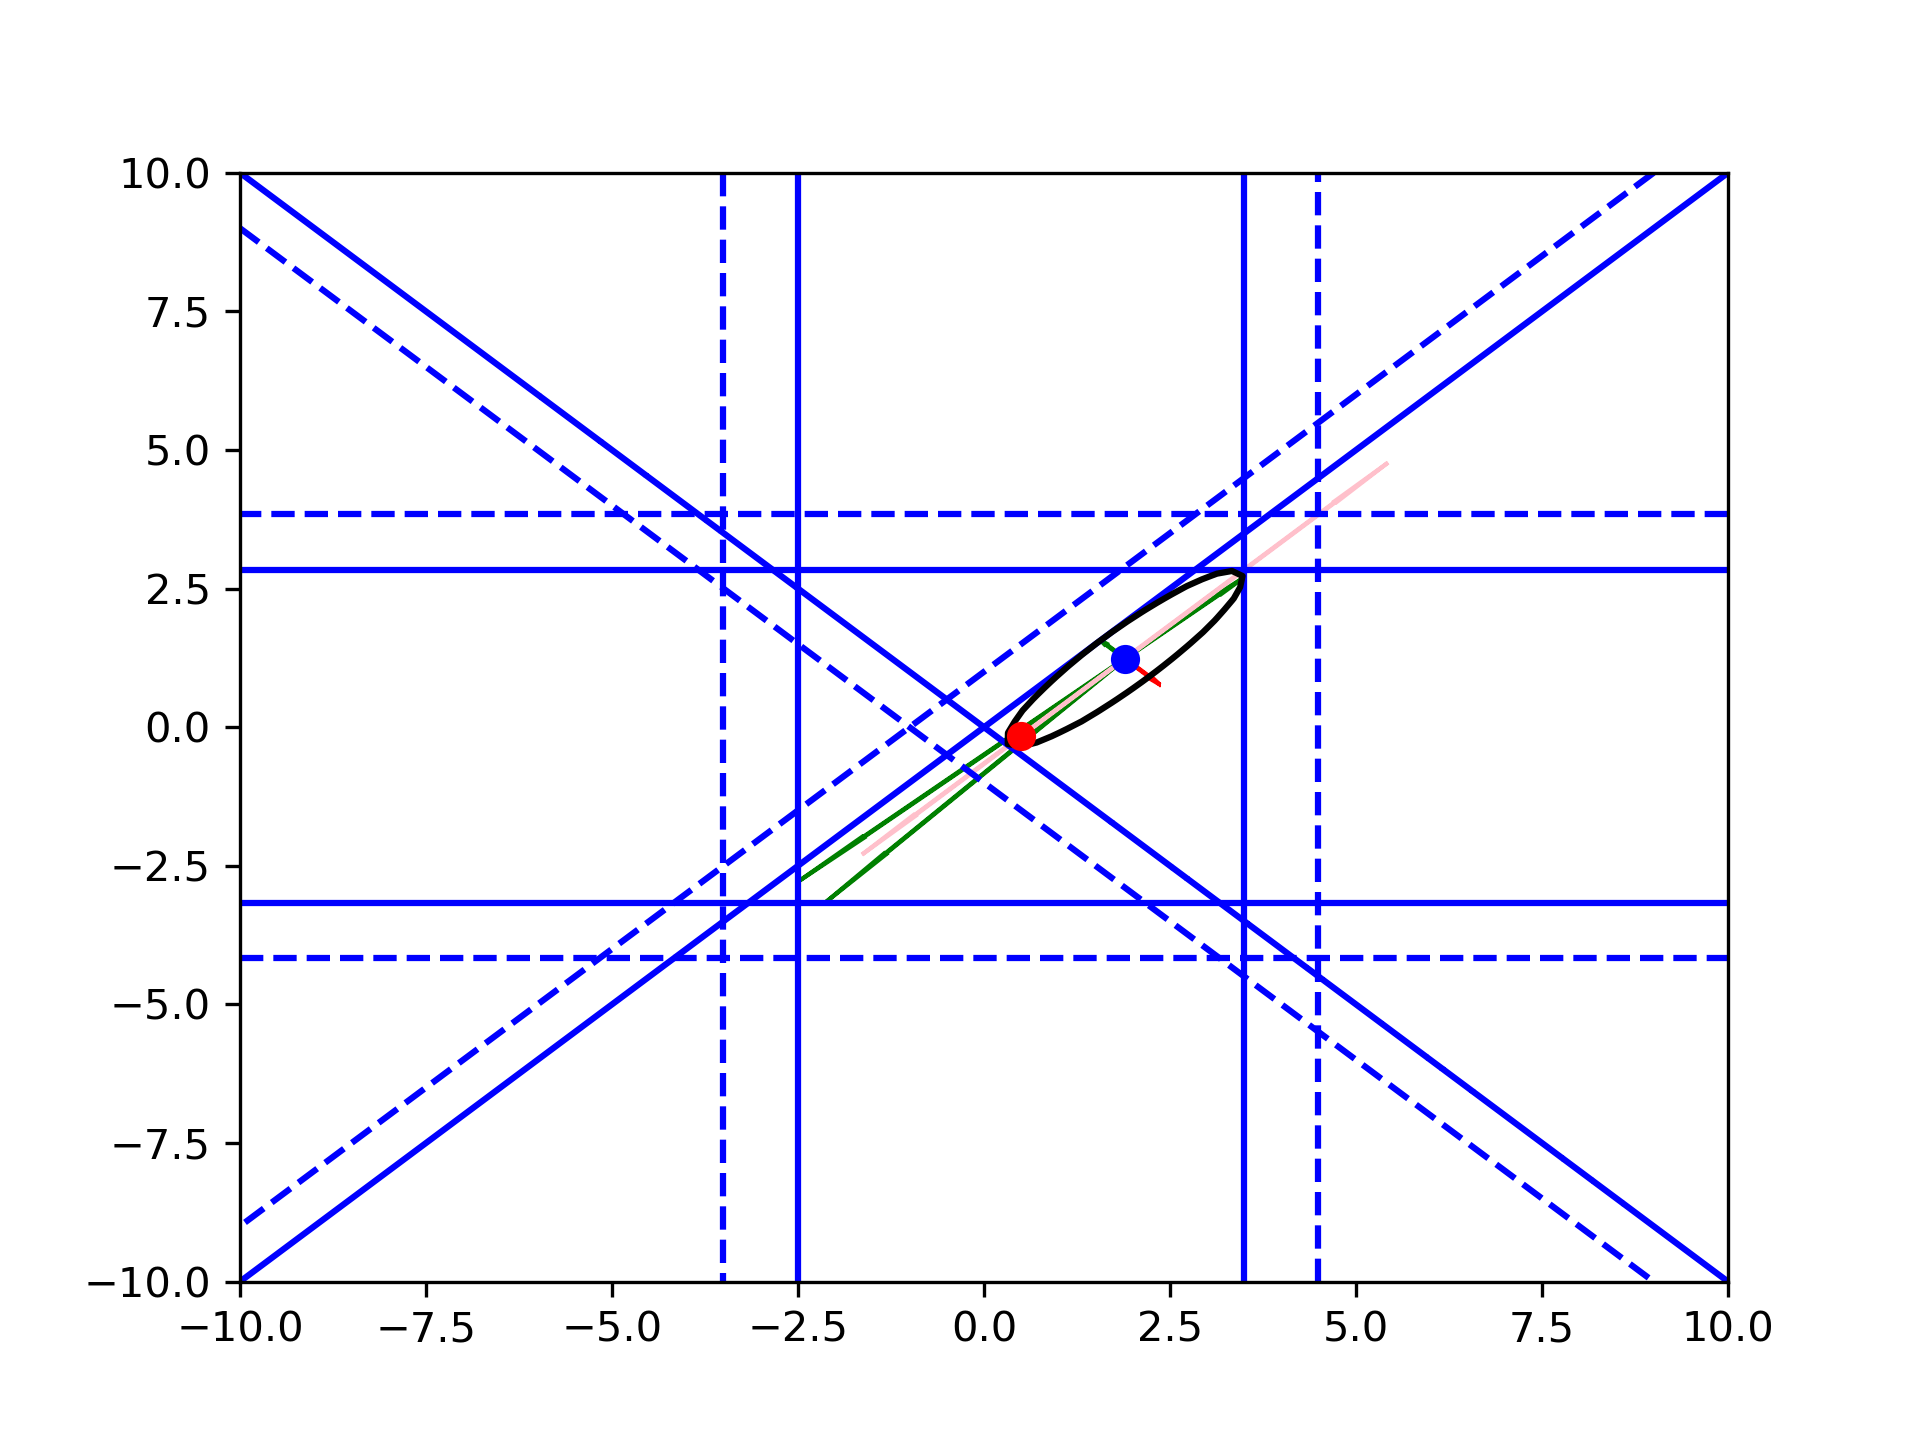
\includegraphics[scale=0.4]{images/line_2.png}
    \caption{Line searches}
    \label{first_line_search}
\end{figure}


For a given distance $d$, let the indices $i$ for which $\frac {|A_i x - b|}{\|A_i\|} \le d$


To fix this, we break the search space within the \emph{ConstructTrustRegion} subroutine into segments based on the nearest constraints.
The algorithm works by chosing a set of up to $n_{\text{points}}$ points $s_1, s_2, \ldots, s_{n_{\text{points}}}$ that are each equidistant to a subset of the constraint's faces.
The center search then considers points along the line segments between these points.
% Namely, it starts at the current iterate and travels along a ray away from all the closest constraints until it reaches a point equidistant to yet another constraint.

More precisely, the first point is chosen to be the current iterate: $s_1 = \iteratek$.
The algorithm then repeats the following process for $i$ from $1$ to $n_{\text{points}}$.
First, compute the set of nearest constraints, where the distance from a point $x$ to a constraint $A_i$ is given by $d(A_i, x) = \frac {|A_i x - b|}{\|A_i\|}$.
While finding the next point $s_{i+1}$, let  $A_E$ be a normalized array of the equidistant faces $\{\frac{A_i}{\|A_i\|} | d(A_i, s_i) = \min_j d(A_j, s_i), i = 1, 2, \ldots, m\}$ and $b_E$ be the rows' corresponding values of $b$.
All other faces are called the remaining faces, and construct the matrix $A_R$ and vector $b_R$.
It then finds a search ray $r{A_E}^T$ as a linear combination of these faces.
When the constraint violation of $s_i$ is non-zero, this search ray can be found by finding the point that doubles the current slack ${A_E}s_i-{b_E}$.
This is given by $r{A_E}^T$ where $r$ solves the linear system ${A_E}(n_i + r{A_E}^T) - b_E = 2 ({A_E}n_i - b_E)$.
If the current violation is zero, then the right hand side can be set to a vector of all ones to ensure that all slacks violations are the same: $A_E(n_i + r{A_E}^T) - b_E = 1$.
We can travel along this ray until we reach a point that is the same distance to a remaining face.
We can travel by 
\begin{align}
t = \argmin_j {\frac{d({A_E}_0, s_i) - d({A_R}_j, s_i)}{ ({A_R}_j - d({A_E}_0) r{A_E}^T} | ({A_R}_j - d({A_E}_0) r{A_E}^T > 0 }. 
\end{align}

We can then set $s_{i+1} = s_{i} + tr{A_E}^T$.

Of course, $n_{\text{points}}$ must be less than or equal to $n + 1$ in order for this to be defined.
Also, the algorithm must stop early, if $A_E$ contains parallel faces.

% if we let $\nabla \modelconstrainti(\iteratek) = A_i$ be the $i$th row of $A$, then we define the distance from a search point $s$ so the $i$th constraint to be


This means that we can define a class of searches that each limit the number of line segments to search $n_{\text{points}}$.

In figure \cref{line_can_run}, the red line shows the line segments equidistant their closest constraints.
Notice that with two line segments, the algorithm can already choose new centers further from the vertex.

% TODO: REPLACE PICTURES
\begin{figure}[h]
    \centering
    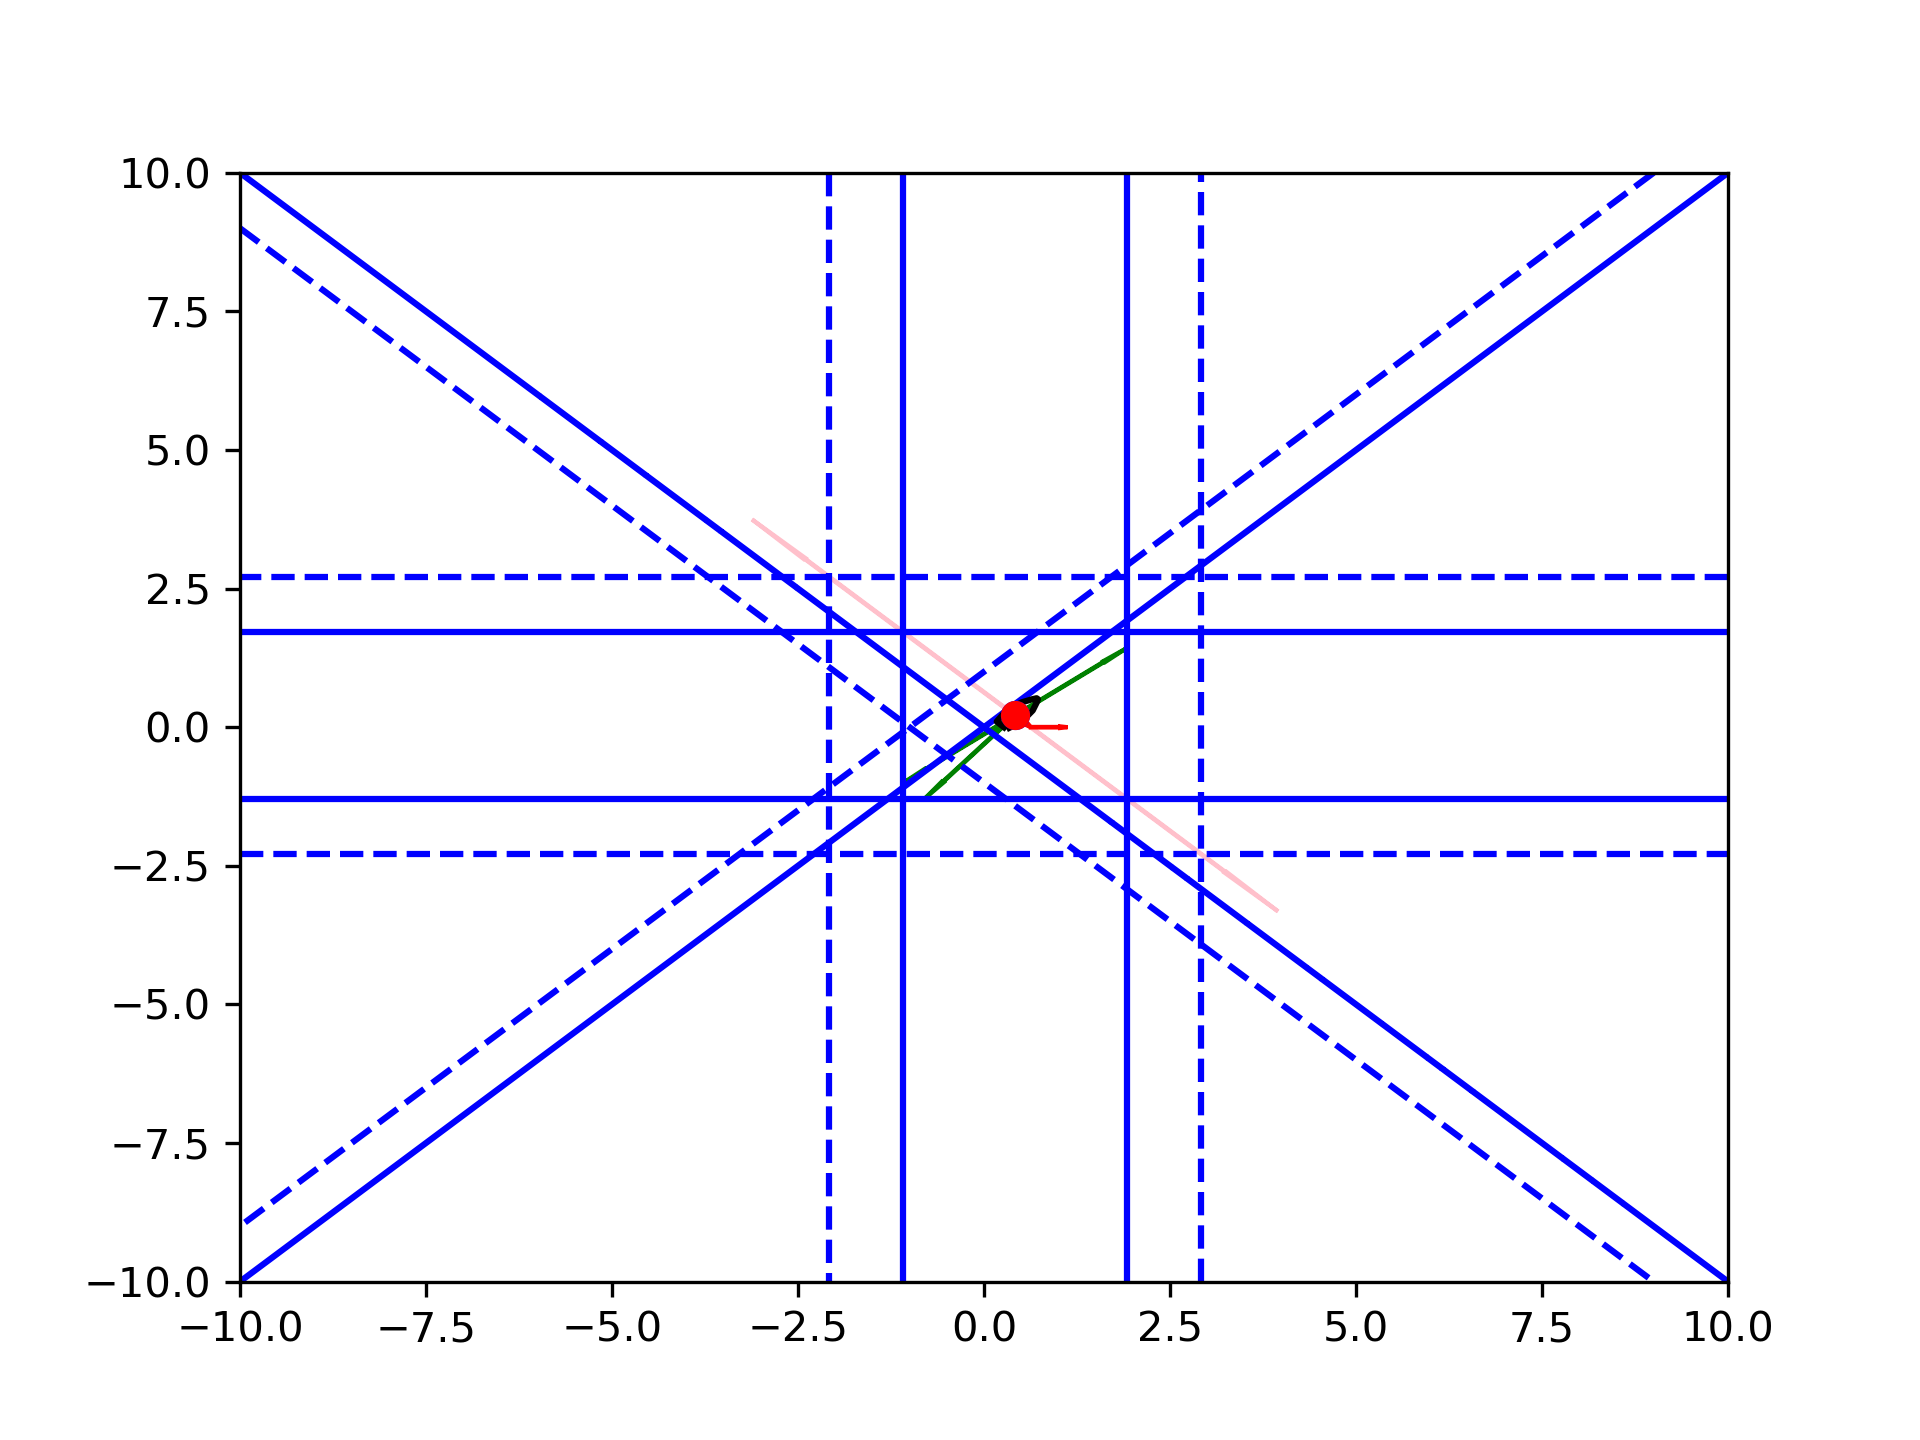
\includegraphics[scale=0.4]{images/run_away_1.png}
    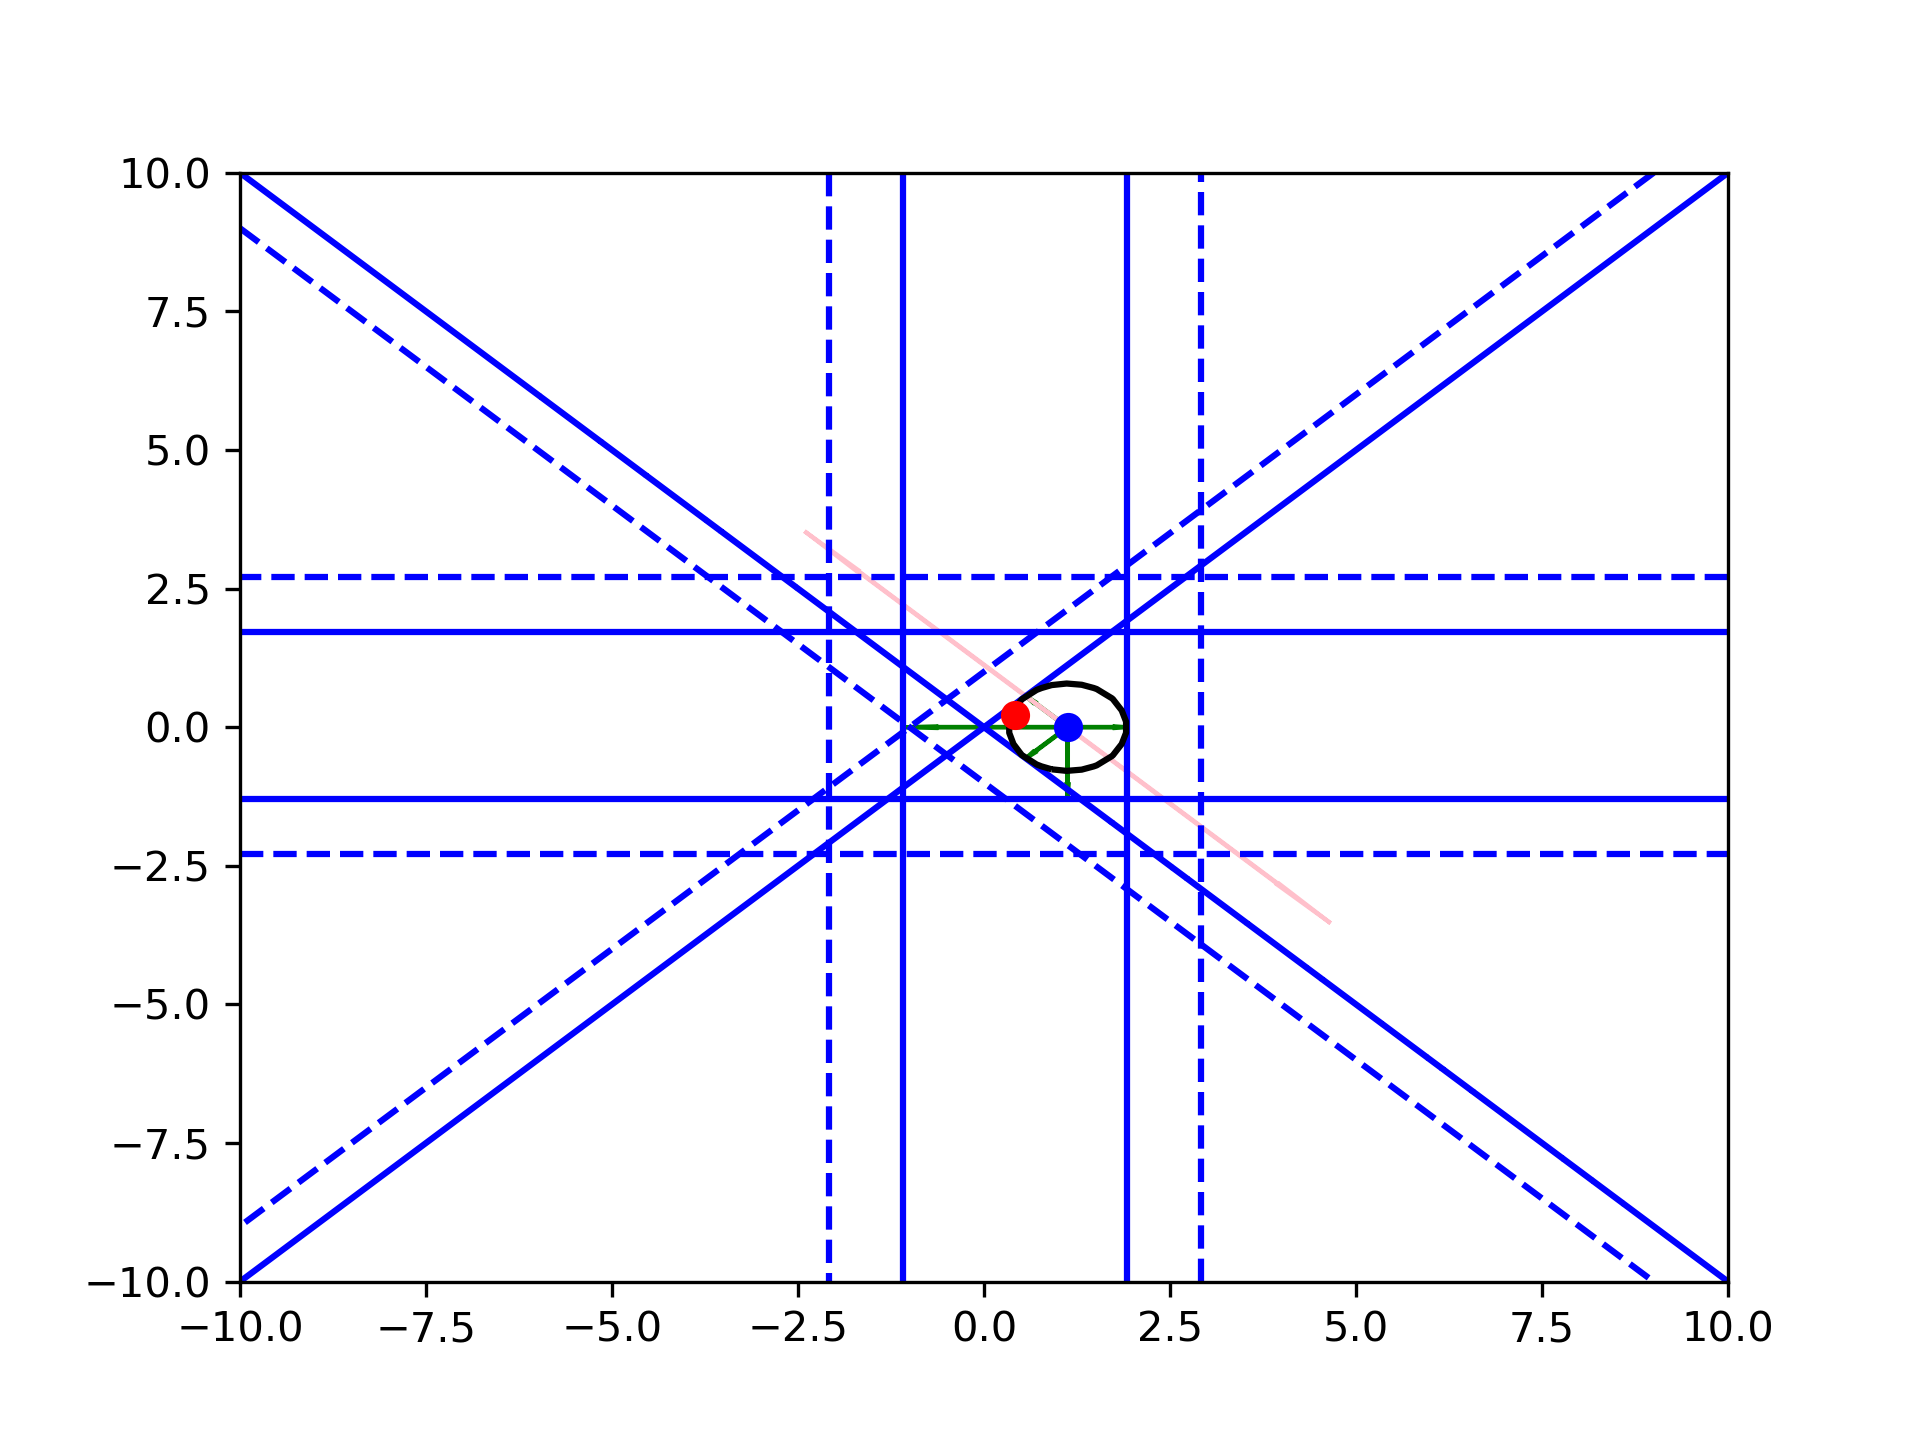
\includegraphics[scale=0.4]{images/run_away_2.png}
    \caption{Ellipse runs away from the optimizer}
    \label{line_can_run}
\end{figure}




